\documentclass[cn,10pt,math=newtx,color=blue]{elegantbook}
% \input{package/package_setup}
\usepackage{listings}
% 用来设置附录中代码的样式
% \lstset{
%     basicstyle          =   \ttfamily,          % 基本代码风格
%     keywordstyle        =   \bfseries,          % 关键字风格
%     commentstyle        =   \rmfamily\itshape,  % 注释的风格,斜体
%     stringstyle         =   \ttfamily,  % 字符串风格
%     flexiblecolumns,                % 别问为什么,加上这个
%     numbers             =   left,   % 行号的位置在左边
%     showspaces          =   false,  % 是否显示空格,显示了有点乱,所以不现实了
%     numberstyle         =   \zihao{-5}\ttfamily,    % 行号的样式,小五号,tt等宽字体
%     showstringspaces    =   false,
%     captionpos          =   t,      % 这段代码的名字所呈现的位置,t指的是top上面
%     frame               =   lrtb,   % 显示边框
% }

\lstset{
    basicstyle=\tt,
    keywordstyle=\color{purple}\bfseries,
    % identifierstyle=\color{brown!80!black},
    commentstyle=\color{gray}
    showstringspaces=false,
}

\lstdefinestyle{Python}{
    language        =   Python, % 语言选Python
    basicstyle      =   \zihao{-5}\ttfamily,
    numberstyle     =   \zihao{-5}\ttfamily,
    keywordstyle    =   \color{blue},
    keywordstyle    =   [2] \color{teal},
    stringstyle     =   \color{magenta},
    commentstyle    =   \color{red}\ttfamily,
    breaklines      =   true,   % 自动换行,建议不要写太长的行
    columns         =   fixed,  % 如果不加这一句,字间距就不固定,很丑,必须加
    basewidth       =   0.5em,
}

\definecolor{mGreen}{rgb}{0,0.6,0}
\definecolor{mGray}{rgb}{0.5,0.5,0.5}
\definecolor{mPurple}{rgb}{0.58,0,0.82}
\definecolor{backgroundColour}{rgb}{0.95,0.95,0.92}

\lstdefinelanguage{CAPL}
{
    morekeywords={byte, dword, }, %定义关键字
    sensitive=false, %是否大小写敏感
}

\lstdefinestyle{C}{
    backgroundcolor=\color{backgroundColour},   
    commentstyle=\color{mGreen},
    % keywordstyle=\color{magenta},
    numberstyle=\tiny\color{mGray},
    stringstyle=\color{mPurple},
    % basicstyle=\footnotesize,
    breakatwhitespace=false,         
    breaklines=true,                 
    captionpos=b,                    
    keepspaces=true,                 
    numbers=left,                    
    numbersep=5pt,                  
    showspaces=false,                
    showtabs=false,                  
    tabsize=4,
    language=C
}

\usepackage{hyperref}
\newcommand{\tabincell}[2]{\begin{tabular}{@{}#1@{}}#2\end{tabular}}
\title{学习笔记}
% \subtitle{Elegant\LaTeX{} 经典之作}

\author{Wang Haojiang}
% \institute{Elegant\LaTeX{} Program}
\date{Dec 1, 2021}
\version{1.0}
\bioinfo{自定义}{信息}

% \extrainfo{各人自扫门前雪,休管他人瓦上霜。—— 陈元靓}

\setcounter{tocdepth}{3}

\logo{logo-blue.png}
\cover{cover.jpg}
\definecolor{customcolor}{RGB}{32,178,170}
\colorlet{coverlinecolor}{customcolor}

\begin{document}
	\maketitle
	\frontmatter
	\tableofcontents
	\mainmatter
	\include{ch1/chapter1}
	\chapter{以太网配置}
\section{NVM}
\subsection{Ram Block}
\subsubsection{Permanent and non-permanent RAM Blocks}
RAM block 可以是永久性的,也可以是非永久性的。永久 RAM 块是只能由一个应用程序访问的 NV 块。 RAM 块的地址是固定的,并存储在 NVM 的配置中。

也可以让多个应用程序访问同一个 NV 块。每个应用程序都使用自己的 RAM 块。在这种情况下,RAM 块称为非永久性的。
由于 RAM 地址未存储在 NVM 配置中(并且可能会变化),因此必须提供一个指针来读取和写入非永久性块。这也是 \lstinline{NVM_WriteALL} 和 \lstinline{NVM_ReadAll} 使用第二个参数传递
非永久 RAM block 地址的原因。

\begin{remark}
异步 API 函数可以由不同的任务重入。因此,多个任务可能同时将 Block 入队,例如写入 job(具有较高优先级的任务可能会中断较低的任务)。
但是不可能将同一个块多次入队(既不能是由不同的任务也不能是由不同的 job)。
因此,例如,如果块 5 的读取作业已排队,则该块的擦除 job 不能在读取 job 完成之前排队。
如果一个块被多个任务使用,这是非永久性 RAM 块的常见任务,应用程序负责同步。当然,例如,如果正在处理擦除请求,则可以读取或写入 RAM 块,而不会对擦除作业的结果产生任何影响。
唯一的问题是 NVM 不向应用程序提供任何信息,即当前正在为块处理什么服务。启动服务的应用程序当然知道,但也使用该块的不同应用程序不知道。
因此,只要块处于挂起状态,这时访问最安全的方法是不要使用 RAM 块。这样可以彻底避免 RAM 不一致。
\end{remark}

\begin{definition}[\lstinline{NvMBlockUseSyncMechanism}]
此参数定义是否为此块使用具有 RAM 镜像和回调例程的显式同步机制,用于将数据传输到 NvM 模块的 RAM 镜像和从 NvM 模块的 RAM 镜像传输数据。
如果使用, \lstinline{NvMReadRamBlockFromNvCallback} 和 \lstinline{NvMWriteRamBlockToNvCallback} 都必须设置为适当函数的名称。
\end{definition}
\begin{definition}[\lstinline{NvMWriteRamBlockToNvCallback}]
  该参数定义了块特定的回调例程,为了让应用程序将数据从 RAM 块复制到 NvM RAM块的镜像,应调用该回调例程。
\end{definition}

\begin{definition}[\lstinline{NvMReadRamBlockFromNvCallback}]
  该参数定义了块特定的回调例程,为了让应用程序将数据从 NvM 模块的镜像复制到 RAM 块,应调用该回调例程。
\end{definition}

NVM 模块支持在应用程序和 NVM间的显式同步机制。实现方式为在 NVM 模块中添加一个 RAM 镜像块。数据在应用程序和NVM模块间通过回调函数进行双向传递,这些回调函数由 NVM模块调用。

每个 Block块可以支持独立配置同步机制。如果配置了同步机制,NVM 模块使用内部 buffer 用作 RAM 块镜像。同样,该块也用于 CRC 计算。buffer 的大小为最大配置 Block 大小加上 CRC 大小。\textbf{实际上大小设置为 256}。如下:

\begin{lstlisting}[language=C,style=C]
  // internal buffer size 
#define NVM_INTERNAL_BUFFER_LENGTH            256uL

// create the internal buffer of size NVM_INTERNAL_BUFFER_LENGTH
VAR(uint8, NVM_PRIVATE_DATA) NvM_InternalBuffer_au8[NVM_INTERNAL_BUFFER_LENGTH];
\end{lstlisting}

为使用同步机制的块配置永久 RAM 块是没有用的。在这种情况下,RAM 块将被忽略。也不建议为使用同步机制的块配置 Init 回调。

\begin{remark}
  如果为块配置了显式同步,则客户端可以在块挂起时修改各自的 RAM 内容(对 NVM 不可见)。在这种情况下,当挂起的读取完成时,请注意它们的值可能会被覆盖。
\end{remark}

\subsubsection{Explicit synchronization mechanism during write requests}
在应用程序发出 \lstinline{NvM_WriteBlock} 后,应用程序可能会修改 RAM 块,直到 NvM 调用回调 \lstinline{NvMWriteRamBlockToNvM} 。
如果调用 \lstinline{NvMWriteRamBlockToNvM} ,应用程序必须向内部 RAM 镜像提供 RAM 块的一致副本。

\subsubsection{Explicit synchronization mechanism during read requests} 
在应用程序发出 \lstinline{NvM_ReadBlock} 后,应用程序可能会修改 RAM 块,直到 NvM 调用例程 \lstinline{NvMReadRamBlockFromNvM} 。
如果调用 \lstinline{NvMReadRamBlockFromNvM} ,则应用程序必须将数据从内部 RAM 镜像复制到 RAM 块。

\subsection{Rom Block}

Rom Block的值由应用程序提供,同样,可以通过初始化回调函数用于提供 Rom 默认值。这些通过配置实现。当然,只可以选择 Rom Block 和 初始化回调函数的其中一种。

Rom 默认值可以通过显式接口调用 \lstinline{NvM_RestoreBlockDefaults()}。在读请求时,也可以隐式的读取默认值。
如以下场景:当从 NVM 存储中没有读取到有效数据,比如由于 CRC 错误或由于底层模块 \lstinline{MEMIF} 报出错误时。

在 block 读操作时,重载了 Rom 默认值,则 block 结果为 \lstinline{NVM_REQ_RESTORED_FROM_ROM}。
直接调用 \lstinline{NvM_RestoreBlockDefaults()} 并不会给出 \lstinline{NVM_REQ_RESTORED_FROM_ROM} 的结果。

\begin{remark}
  上面所说的结果可以通过以下接口获取:
  \begin{lstlisting}[language=C,style=C]
  Std_ReturnType NvM_GetErrorStatus ( NvM_BlockIdType BlockId,  NvM_RequestResultType* RequestResultPtr)
  \end{lstlisting}
\end{remark}

\subsection{The configuration ID}

block 1 NvMConfigBlock是一个特殊的 NV 块,其保存了一个常量\lstinline{NvM_CompiledConfigId_t},该常量和配置项\lstinline{/MICROSAR/NvM/NvMCommon/NvMCompiledConfigId}对应。当\lstinline{ReadAll}时,该Block的值和常量值进行比较,当两个值匹配时,所有的NV
block可认为是有效的,NVM尝试从NV中读取数据。如果值不匹配或者没有读取到有效的configuration ID,则NVM的系统行为如下:

\begin{itemize}
	\item
  当配置项\lstinline{/MICROSAR/NvM/NvMCommon/NvMDynamicConfiguration}为 off 时,不匹配将被忽略,NVM将从NV中尝试读取数据。(normal runtime preparation)。
	\item
  当配置项为on时,所有配置了\lstinline{/MICROSAR/NvM/NvMBlockDescriptor/NvMResistantToChangedSw}的block,将视为 normal runtime preparation,将从NV中尝试读取数据。其他未配置的block将视为 extended runtime preparation。不会从NV中读取数据。
	\item
  所有视为 extended runtime preparation 的block,将被认为是无效的或空的block。因此,配置为 write once 的block将被重写。如果配置了 rom block 或初始化回调函数,则会进行值的初始化。
\end{itemize}

\subsection{Block状态查询}

\subsubsection{\lstinline{NvM_QryBlockRelevantForWriteAll}}

block在满足以下条件后,writeall 阶段可写入NV Block。

\begin{itemize}
\item
  block勾选了 \lstinline{Write all}

  \begin{itemize}
  \item
    使能
    \lstinline{NVM_SET_RAM_BLOCK_STATUS_API}时,当block状态为\lstinline{NVM_STATE_CHANGED_SET}和\lstinline{NVM_STATE_VALID_SET}时,需要写入,否则无需写入。
  \item
    未使能 \lstinline{NVM_SET_RAM_BLOCK_STATUS_API}时,需要写入。
  \end{itemize}
  
\item
  未勾选 \lstinline{Write all},无需写入。
\end{itemize}

\subsubsection{\lstinline{NvM_ApiFlags}}

\begin{figure}
\centering
\includegraphics{./pic/NvM_ApiFlags.png}
\caption{nvm-01}
\end{figure}


\subsubsection{readall 和 writeall顺序}

\begin{itemize}
\item
  Write all从block id最大值的到0
\item
  Read all 从0到 id最大值
\end{itemize}

\subsection{CRC机制}

\subsubsection{NvMCalcRamBlockCrc}
% 全局ram block的CRC是否需要计算或重新计算。在\lstinline{Read all}阶段,NVM内部存储读到的CRC值,并进行数据校验和比较。
\begin{remark}
  目前的理解是,NVM 模块通过内部的 CRC buffer 存储 block 的 CRC 值,并在 \lstinline{NVM_ReadAll} 阶段,验证 Ram block 的 CRC值是否一致,一致时避免从NV 中读数据。
\end{remark}

NvMCalcRamBlockCrc 配置影响下的处理流程,如下图所示:

\begin{figure}[ht]
  \centering
  \includegraphics[scale=0.35]{pic/NVM_cal_ram_crc.png}
  \caption{NvMCalcRamBlockCrc 处理流程}
  \label{fig:NVM_cal_ram_crc}
\end{figure}

对于某些 NVRAM 块,可能需要在 \lstinline{NvM_ReadAll} 期间保护相应 RAM 块的数据内容不被覆盖,以防存储在相应 NV 块中的数据比 RAM 块中的数据更旧。例如以下场景,当 RAM 中的数据尚未写入 NV 存储器时热复位。
在这种情况下,RAM 块必须分配在复位安全(不经历初始化)的 RAM 区域中,并且配置参数 CalcRamBlockCrc 必须设置为 \lstinline{TRUE}。 这意味着相应的 NV 块也具有/具有 CRC 配置,并且参数 \lstinline{NvMSetRamBlockStatus} Api 必须设置为值 \lstinline{TRUE} 。

每次更改 RAM 块数据内容后,必须为相应的 NVRAM 块调用 API \lstinline{NvMSetRamBlockStatus} ,并将参数 \lstinline{BlockChanged} 设置为 \lstinline{TRUE} 。然后,NVM 将重新计算此 RAM 块的 CRC,并将结果存储在分配在复位安全(不经历初始化)RAM 区域中的内部变量中。
作为此 NVRAM 块的先决条件,必须配置有效的永久 RAM 块 (NvMRamBlockDataAddress) 或显式同步回调函数 (NvMReadRamBlockFromNvM)。

在每次启动 (\lstinline{NvM_ReadAll}) 期间,NvM 模块都会计算此类 RAM 块的 CRC,如果它与存储的 CRC 值匹配,则不会覆盖 RAM 块。如果计算出的 CRC 与存储的 CRC 不匹配,RAM 块将被从 NV 块读取的数据覆盖,或者,如果此读取尝试失败,
使用默认数据恢复(如果通过参数 NvMRomBlockDataAddress 或参数 NvMInitBlockCallback 配置)。

\subsubsection{NvMBlockUseCrc}
block是否使用CRC。


\subsubsection{NvMBlockUseCRCCompMechanism}

block是否使用compare mechanism。

如果特定ram block对应的NV data在运行时没有更新,为了避免不必要的 NV 写操作,提供了compare
mechanism机制。即,在向NV写数据之前,重新计算当前ram数据的CRC值,并和之前读或写数据操作时保存的CRC值进行比较。

\subsubsection{NvMCrcIntBuffer}

NVM是否内部分配buffer用于CRC校验处理,如果不开启,则每个ram block需要应用程序为各 block 提供空间存储CRC。
当开启内部buffer后,用户数据被拷贝至buffer,然后附加上CRC信息,最后一起被送至下层模块处理。

% \subsubsection{异步 CRC 计算}
% Block 的CRC 值总是在 \lstinline{NvM_MainFunction}中异步计算。
% 当要写入一个Block 到NV 中,则Block 块的 CRC 值总要提前计算。如果读取一个 block,则读取数据的 CRC 值会重新计算并和 NV 中存储的 CRC 值和存储在其他地方的值进行比较。
% 如果一个 Block 勾选了配置 NvMCalcRamBlockCrc ,则其最近计算的 CRC 值将存储在 RAM 中供以后使用。在此配置下,如果一个 block 调用了
% \lstinline{NvM_SetRamBlockStatus(TRUE)}, 则 Ram block 的CRC 值将重新计算。

\subsubsection{异步CRC校验}

block对应的CRC校验是在\lstinline{NvM_MainFunction}中异步进行的。受CRC保护的block在写数据到NV前,都需要计算CRC值。如果从NV中读取数据,CRC的值需要重新计算并和读取到的CRC值进行比较。如果配置了\lstinline{NvMCalcRamBlockCrc},最近计算到的CRC值将存储在RAM中,便于后续使用。

如果调用了
\lstinline{NvM_SetRamBlockStatus(TRUE)},且为此块启用了\lstinline{NvMCalcRamBlockCrc},则还将启动对RAM块数据的CRC值的重新计算。

NvM 在 \lstinline{NvM_ReadAll} 处理期间尝试对所有在其配置中启用了 \lstinline{Read during ReadAll} 和 \lstinline{Calc RAM CRC} 的
NVRAM 块进行尝试:如果块在内部仍标记为 VALID,NVM 将计算当前 RAM
块内容的 CRC 值和存储在其他地方的值进行比较。 如果它们匹配,则不会触及
RAM 内容; 相反,NVM 假装已成功从 NV 读取这些值。

\begin{itemize}
\item
  如果匹配,则无需写操作,并成功结束任务。
\item
  如果不匹配,则需要向NV中写数据。
\end{itemize}

CRC Compare Mechanism和 NvMCalcRamBlockCrc
没有依赖关系,这两者各自使用独立的CRC buffer。

\begin{itemize}
\item
  NvMCalcRamBlockCrc:
  调用 \lstinline{NvM_SetRamBlockStatus} 将引起CRC值的重新计算,NVM保存当前ram
  block数据的CRC值,并在read all时避免真实的从NV
  中读取数据。详见 异步CRC校验。
\item
  Compare Mechanism:
  NVM保存上一次成功读取或写入数据对应的CRC值,如果该CRC值与ram
  block的数据CRC值匹配,则调用\lstinline{NvM_WriteBlock, NvM_WriteAll}时可避免不必要的数据写入。
\end{itemize}

\subsection{API 分析}
\subsubsection{\lstinline{NvM_QueuePop}}

从 Queue 中 pop 第一个job, job 的索引值作为参数返回,入口参数为指针,同样,原 Queue 将指向 pop 元素的下一个元素。

\begin{lstlisting}[language=C,style=C]
  /**********************************
  * NvM_QueuePop
  ***********************************/
 /*! \brief Removes first element from queue.
  *  \details Pops the first element from the given list, i.e. the element is removed from the list and will be returned.
  *           The given list shall not be empty!
  *  \param[in,out] Queue as an index to the queue to pop out of the queue. Caller has to ensure validity.
  *  \return given element's index
  *  \context TASK
  *  \reentrant FALSE
  *  \synchronous TRUE
  *  \config Configuration class is > 1
  *  \pre -
  */
NVM_LOCAL FUNC(NvM_QueueEntryRefType, NVM_PRIVATE_CODE) NvM_QueuePop(NvM_QueueListHeadRefType Queue);
\end{lstlisting}

\subsubsection{\lstinline{NvM_QueuePush}}
在 Queue 中 push 一个元素,队列的第一个元素变为刚入栈的元素。

\begin{lstlisting}[language=C,style=C]
  /**********************************
  * NvM_QueuePush
  ***********************************/
 /*! \brief Add job to queue.
  *  \details Pushes the given element onto the given list, i.e. the element is inserted at list head.
  *  \param[in] Queue as an index to the next queue element. Caller has to ensure validity.
  *  \param[in] Elem as an index to the queue, shall be enqueued at the end of the linked list.
  *             Caller has to ensure validity.
  *  \context TASK
  *  \reentrant FALSE
  *  \synchronous TRUE
  *  \config Configuration class is > 1
  *  \pre -
  */
 NVM_LOCAL FUNC(void, NVM_PRIVATE_CODE) NvM_QueuePush(NvM_QueueListHeadRefType Queue, NvM_QueueEntryRefType Elem);
\end{lstlisting}

\subsubsection{\lstinline{NvM_ActGetNormalPrioJob}}
取出 有效 job queue,即 \lstinline{NvM_NormalPrioQueue.SrvList} 中最先入栈的 job ,并将该 job 的信息保存到 \lstinline{NvM_CurrentJob_t}中。
之后有效队列继续指向最先入队的 job。空队列则入栈一个 job 空位。

\begin{lstlisting}[language=C,style=C]
  /**********************************
  * NvM_ActGetNormalPrioJob
  ***********************************/
 /*! \brief Setups the NvM internal job variable for next job.
  *  \details Scans the given queue for the entry with highest priority, located nearest to the list end.
  *           The element is removed from the list, but stored in NvM_lastJobEntry. The job parameters will be copied
  *           to the passed job structure. The queue is expected to contain at least one element.
  *  \context TASK
  *  \reentrant FALSE
  *  \synchronous TRUE
  *  \config Configuration class is > 1
  *  \pre -
  */
  FUNC(void, NVM_PRIVATE_CODE) NvM_ActGetNormalPrioJob(void)
  {
      NvM_QueueEntryRefType elem;
  
      NvM_EnterCriticalSection();
      /* just take the last queue element, don't store it in NvM_LastJobEntry (it does not exist),
       * but remove it from the queue.
       * Just update the queue head to point to its prev element (which is the tail), then pop.
         After that, the head points to the head again.
       */
      NvM_NormalPrioQueue.SrvList = NvM_JobQueue_at[NvM_NormalPrioQueue.SrvList].PrevEntry;
      elem = NvM_QueuePop(&NvM_NormalPrioQueue.SrvList); /* SBSW_NvM_FuncCall_PtrParam_Queue */
  
      /* free the element --> add it to free-list */
      NvM_QueuePush(&NvM_NormalPrioQueue.EmptyList, elem); /* SBSW_NvM_FuncCall_PtrParam_Queue */
  
      NvM_CurrentJob_t.JobBlockId_t = NvM_JobQueue_at[elem].BlockId;
      NvM_CurrentJob_t.JobServiceId_t = NvM_JobQueue_at[elem].ServiceId;
      NvM_CurrentJob_t.RamAddr_t = NvM_JobQueue_at[elem].RamAddr_t;
  
  
      NvM_ExitCriticalSection();
  }
\end{lstlisting}
\section{网络层}
\subsection{组播}
\subsubsection{组播地址}

组播报文的目的地址使用D类IP地址, D类地址不能出现在IP报文的源IP地址字段。

单播数据传输过程中,一个数据包传输的路径是从源地址路由到目的地址,利用“逐跳”的原理在IP网络中传输。

然而在ip组播环中,数据包的目的地址不是一个,而是一组,形成组地址。

所有的信息接收者都加入到一个组内,并且一旦加入之后,流向组地址的数据立即开始向接收者传输,组中的所有成员都能接收到数据包。
组播组中的成员是动态的,主机可以在任何时刻加入和离开组播组。

\subsubsection{范围}

\begin{itemize}
    \item 224.0.0.0~224.0.0.255为预留的组播地址(永久组地址),地址224.0.0.0保留不做分配,其它地址供路由协议使用;
    \item 224.0.1.0~224.0.1.255是公用组播地址,可以用于Internet;
    \item 224.0.2.0~238.255.255.255为用户可用的组播地址(临时组地址),全网范围内有效;
    \item 239.0.0.0~239.255.255.255为 \textbf{本地} 管理组播地址,仅在特定的本地范围内有效。

\end{itemize}

\subsubsection{组播IP地址和MAC地址转换}

组播MAC地址有IP地址映射转换而成,过程如下图所示:

\begin{figure}[ht]
    \centering
    \includegraphics[scale=0.7]{pic/multicast-01.png}
    \caption{multicast ip addr to mac}
    \label{fig:multicast_ip_addr_to_mac}
\end{figure}


过程如下:

\begin{enumerate}
    \item 加上MAC地址固定前缀(24bit)为:01-00-5E;
    \item 后面24bit由IP地址的后23bit构成;
    \item 第25 bit位固定为0;
\end{enumerate}

\subsubsection{举例}

以Someip SD服务组播地址为例,组播IP地址为 \textbf{239.127.3.1}。

\begin{itemize}
    \item 二进制: \textbf{1110 1111 0111 1111 0000 0011 0000 0001}
    \item 固定前缀: \textbf{01-00-5E- + 0b}
    \item 转换结果: \textbf{01-00-5e-7f-03-01}
\end{itemize}

\subsubsection{代码实现}

协议栈中由TCPIP模块分配多播IP地址到设置 \lstinline{ENET} multicast mac filter \lstinline{ENETn_GAUR/GALR}寄存器的过程如下图所示:

\begin{figure}[h]
    \centering
    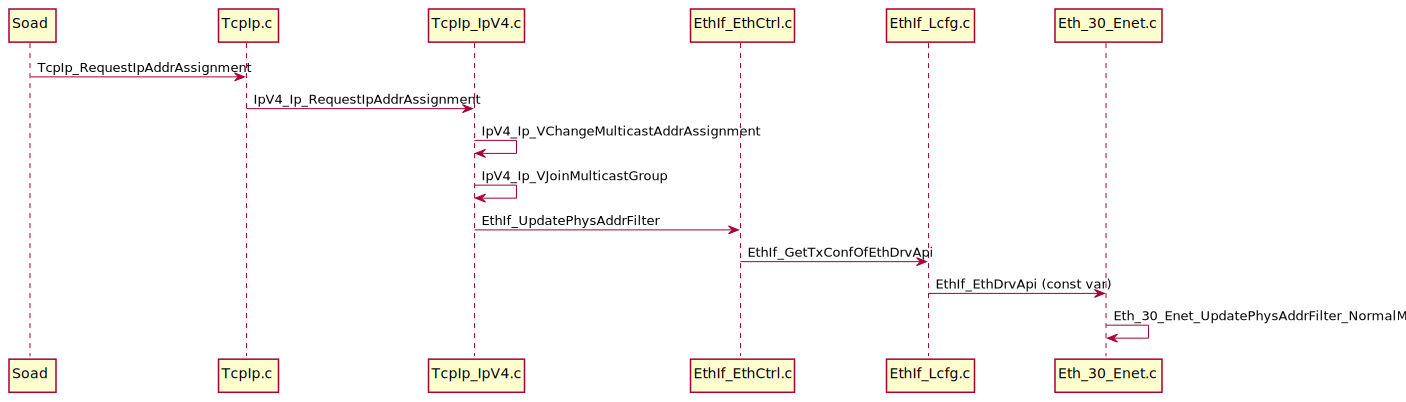
\includegraphics[scale=0.5]{pic/eth_multicast_mac_code.pdf}
    \caption{eth multicast mac code}
    \label{fig:eth_multicast_mac_code}
\end{figure}
\section{CANoe 以太网工程配置}
本节基于vector vn5620 硬件,对 CANoe 软件中以太网相关的配置方法进行总结。

\subsection{工程配置---Network-based Access}
硬件设备从固件版本 11.1 后,支持新的以太网配置方式,称为 Network-based Access。新固件下支持以下功能:

\begin{itemize}
    \item 网络和端口定义
    \item 自由的设备分片
    \item 以太网接口-PC 连接
    \item 硬件过滤
\end{itemize}
\subsubsection{基础概念}
新的模式下,存在以下几个概念,详细模块如图所示:

\begin{figure}[ht]
    \centering
    \includegraphics[scale=0.7]{pic/Snipaste_2021-10-29_09-46-43.png}
    \caption{术语实例}
    \label{fig:new_terms}
\end{figure}

\begin{enumerate}
    \item Port: 软件或硬件接入设备的入口,所以也分为物理端口和虚拟端口。CANoe 中仿真节点接入的就是虚拟端口。一个端口只能被一个 segment 包含。
    \item Segment: 分片是端口的组合。 必须至少创建一个分片并连接到一个物理端口。 每个分片都有一个唯一的名称,并且恰好分配给一个网络。 有两种类型的段可用:switch 和 link。 
    \begin{enumerate}
        \item switch segment: 提供 2 层交换机的功能。
        \item link segment: 完全透明地连接两个端口。 用于透明地转发以太网数据包和物理层的状态。Link segment 存在两种连接方式:TAP 和 直连。TAP 模式下,两个物理端口间有很小的延迟($\leq 6 \mu s$)。类似之前固件中提供的 MAC 旁路功能。
        直连模式适用于一个物理端口和虚拟端口间的连接。
    \end{enumerate}

    \item Network: 一个网络包括一个或多个分片。硬件设备中至少需要定义一个网络。
    \item Uplink: 设备和 CANoe PC 间的连接称为 uplink,可以通过配置 filter 减少传输给上位机的数据量。
\end{enumerate}

\subsubsection{概念变更}

\begin{figure}[ht]
    \centering
    \includegraphics[scale=0.7]{pic/Snipaste_2021-10-29_14-37-48.png}
    \caption{拓扑实例}
    \label{fig:example_topology}
\end{figure}
图\ref{fig:example_topology} 包含两个复杂网络节点 \textbf{N3} 和 \textbf{N4},各自集成了一个 switch。
另外每个 switch 上连接了一个仿真节点 \textbf{N1} 和  \textbf{N6}。两个真实节点  \textbf{N2} 和  \textbf{N5}。

下图 \ref{fig:two_setup} 展示了固件版本 11.1 前后的实现方法。

\begin{figure}[ht]
    \centering
    \includegraphics[scale=0.6]{pic/Snipaste_2021-10-29_14-42-44.png}
    \caption{ Simulation setup of the device firmware before version 11.1 vs. simulation setup of the device firmware from version 11.1}
    \label{fig:two_setup}
\end{figure}

之前版本中,一个设备仅能配置一个 switch 分片,因此,需要两个设备通过两个通道接入 CANoe。所以,在 CANoe 中需要配置两个 network。
之后版本中,允许自由配置分片。因此,可以配置两个 switch 分片,两个分片都分配在一个 network 中。因此,在 CANoe 中,仅需要配置一个 network。

\subsubsection{以太网包的收发方向}
设备接口接收到的以太网数据包总是标有 Rx 方向。 在这种情况下,数据包是由应用程序(例如 CANoe 模拟节点)生成还是来自真实网络无关紧要。
从接口发送到真实网络或模拟节点的数据包(例如,由于交换机段中的转发规则)被标记为 Tx 数据包。 
\begin{note}
    简单理解,新的方向,就是以硬件设备自身的角度考虑。从真实节点或仿真节点发给设备的都是 Rx 数据包,从设备发出去的都是 Tx 数据包。
\end{note}

\subsubsection{以太网硬件配置}
以太网硬件接口配置在 \textbf{Vector Hardware Config} 窗口中。如下图所示。
可以打开 \textbf{Ethernet Device Configuration}。

\begin{figure}[ht]
    \centering
    \includegraphics[scale=0.6]{pic/Snipaste_2021-10-29_15-00-01.png}
    \caption{ \textbf{Ethernet Device Configuration} 配置界面}
    \label{fig:Ethernet_Device_Configuration}
\end{figure}

下图\ref{fig:three_connect_ways}展示了三种连接方式,分别为:
\begin{itemize}
    \item 真实节点和仿真节点通过 switch 连接
    \item 真实节点和仿真节点直连
    \item 两个真实节点旁路连接,CANoe 作为检测
\end{itemize}

\begin{figure}[!ht]
    \centering
    \includegraphics[scale=0.5]{pic/Snipaste_2021-10-29_15-06-06.png}
    \caption{三种连接方式}
    \label{fig:three_connect_ways}
\end{figure}

以第三种 TAP 连接方式为例,完成以上配置后,需要对以太网使用通道、通道和 network 映射、端口等进行详细配置。通道使用配置见下图\ref{fig:eth_channel_usage} \footnote{在实际使用中,仅需要使能 1 个通道,否则会报通道分配错误,详见图\ref{fig:eth_channel_usage_error}}。

\begin{figure}[ht]
    \centering
    \includegraphics[scale=0.5]{pic/Snipaste_2021-10-29_15-18-52.png}
    \caption{以太网通道使用配置}
    \label{fig:eth_channel_usage}
\end{figure}

\begin{figure}[!ht]
    \centering
    \includegraphics[scale=1]{pic/Snipaste_2021-10-29_15-22-58.png}
    \caption{以太网通道配置错误}
    \label{fig:eth_channel_usage_error}
\end{figure}

以太网通道映射,需要将以太网通道和 Simulation Setup 中定义的 Network 及 实际硬件配置的 network进行映射。详见图\ref{fig:eth_channel_mapping}。
\begin{figure}[!ht]
    \centering
    \includegraphics[scale=0.5]{pic/Snipaste_2021-10-29_15-25-55.png}
    \caption{以太网通道映射}
    \label{fig:eth_channel_mapping}
\end{figure}

最后,需要对端口状态进行配置,如进行激活等。详见图\ref{fig:port_Configuration}。
\begin{figure}[!ht]
    \centering
    \includegraphics[scale=0.5]{pic/Snipaste_2021-10-29_15-29-21.png}
    \caption{以太网端口配置}
    \label{fig:port_Configuration}
\end{figure}

\subsection{TcpIp 协议栈配置}\label{sec:two_node_comm}
协议栈配置步骤中,主要对TCP/IP协议栈中的IP地址,mac 地址,VLAN 等配置。
以一个真实节点 GW 和一个仿真节点 ECU1 的通信为例,两节点通过 Link Direct 连接。对 ECU1 协议栈的配置如图\ref{fig:tcpip_Configuration}所示。

\begin{figure}[!ht]
    \centering
    \includegraphics[scale=0.5]{pic/Snipaste_2021-10-29_16-08-23.png}
    \caption{以太网协议栈配置}
    \label{fig:tcpip_Configuration}
\end{figure}

\begin{note}
    当需要配置 VLAN 时,仿真节点协议栈中,一定要在 VLAN 详细配置中,添加对应的IP地址,否则,不能正常收发带正确 VLAN tag 的以太网帧,导致仿真结果出错。
\end{note}

\subsection{CAPL 仿真以太网节点}
以第\ref{sec:two_node_comm}节一个真实节点和一个仿真节点的通信为例,仿真节点的 CAPL 代码实现如下。
实现功能为:

\begin{enumerate}
    \item 启动后,发出 0x401 帧唤醒网络,并同时发出 0x459 帧,激活以太网DoIP功能。
    \item 等待 10s后,发起 TCP 握手,建立 TCP 连接。
    \item 等待 20s后,停发唤醒信号和以太网激活信号。
    \item 等待 60s后,网络应当休眠,重启计数器,循环上述过程。
\end{enumerate}
\input{ch2/gw_tbox_simu.tex}

\section{以太网及 DoIP 配置流程}

基于 Vector Davinci 软件完成基本的以太网通信及 DoIP 诊断功能,可按照以下步骤进行配置:

\begin{enumerate}
    \item 添加以太网 Task 和 \lstinline{ctcddethswc} 确保原有工程添加以太网 SWC 后可正常调度, SWC 仅保留 Switch 硬件初始化的代码,其他不要添加。
    \item 添加以太网相关模块,包括协议栈基础模块及其他关联模块。处理所有错误后,仅添加以太网 Rx Tx 中断和以太网通道 comm \lstinline{mainfunction} 映射,确保工程仍正常运行。
    \item 检查 vlinkGen 模块是否有 \lstinline{.EthRam} var section 配置, 如果开启 cache,需要检查是否进行 cache 保护,及 SMPU flash 块的寄存器配置。
    \item 添加以太网初始化函数(BSW), ECUM \lstinline{memoryInit} 初始化函数,确保工程仍正常运行。
    \item 检查 Switch 硬件相关管脚设置,包括 PWMG 模块与 \lstinline{ctcddethswc},确保初始化管脚时序正确。
    \item 对 Switch 初始化函数进行背景任务映射,确保 Switch 可以正常初始化。
    \item 添加 eth 相关模块的 \lstinline{ mainfunction} 映射,修改 BSWM eth comm 通道控制,修改 SWC 以太网通信控制逻辑代码,验证 DoIP功能是否正常(初期需要默认使能激活线,否则无法建立 TCP 连接)。
    \item 修改 \lstinline{EcuM_Callout_Stubs.c} 中关于休眠前,以太网相关寄存器的配置,确保可以正常休眠。
    \item 修改 \lstinline{ctcddethswc} 与 \lstinline{CtApNmAppSwc} 关联接口代码,如 \lstinline{RCtCddEthSwc_EthCommunicationControl} 函数等。确保以太网通信与 CAN 网络管理状态同步。
\end{enumerate} 

接下来的各节分别针对各步骤中的关键配置进行梳理。

\subsection{SWC 基本结构及配置}
\subsection{以太网协议栈模块配置}
\subsection{vlinkGen 以太网相关配置}
\subsection{BSWM ECUM 以太网初始化配置}
\subsection{以太网相关管脚设置}
\subsection{以太网 Switch 初始化}
\subsection{BSWM ECUM 以太网通道使能配置}
\subsection{休眠期以太网寄存器检查}
\subsection{以太网通信控制与 CAN 网络管理同步}

\section{以太网测试}
\subsection{以太网接线}
DoIP本地诊断的接线如图1、2和表1所示,包括RJ45转obd16,obd16内部pin脚定义及GW04m Connect C pin脚定义。

\begin{figure}[ht]
    \centering
    \includegraphics[scale=0.6]{pic/Quicker_20211111_101031.png}
    \caption{obd-RJ45 pin脚定义}
    \label{fig:Quicker_20211111_101031}
\end{figure}

\begin{figure}[ht]
    \centering
    \includegraphics[scale=0.6]{pic/obd_pin.png}
    \caption{obd pin脚定义}
    \label{fig:obd_pin}
\end{figure}

\begin{figure}[ht]
    \centering
    \includegraphics[scale=0.6]{pic/connect_c_pin.png}
    \caption{Connect C pin脚定义}
    \label{fig:connect_c_pin}
\end{figure}

通过如上接线,可实现pc网卡和GW诊断接口的以太网连接,由于RJ45-OBD16的以太网激活线(pin8)和kl30(pin16)经电阻直连,所以实车插入obd后,即可激活DoIP。台架上则需注意供电或直接拉高以太网激活线。

\subsection{Switch端口镜像配置方法}

Switch的端口镜像功能实现将某一指定Port的入口流量(ingress)和出口流量(egress)镜像至另一指定Port,便于switch流量的实时监控。以太网硬件诊断需求中使用DID CE06配置使能switch A各端口的镜像功能,输出镜像流量的Port为Switch A的port6,即本地诊断口。

\begin{figure}[ht]
    \centering
    \includegraphics[scale=0.6]{pic/switch_mirror.png}
    \caption{switch端口镜像功能}
    \label{fig:switch_mirror}
\end{figure}

DID CE06共两字节,各bit控制信息如下表所示:

% Table generated by Excel2LaTeX from sheet 'Sheet1'
\begin{table}[htbp]
    \centering
    \caption{Add caption}
      \begin{tabular}{ccp{7.165em}p{7.165em}p{8.125em}}
      \toprule
      \rowcolor[rgb]{ .651,  .651,  .651} \multicolumn{1}{p{2.585em}}{\textbf{Byte}} & \multicolumn{1}{p{3.71em}}{\textbf{Bite}} & \textbf{Switch port} & \textbf{对应控制器\newline{}(硬件0.66)} & \textbf{对应控制器\newline{}(硬件0.66之前版本)} \\
      \midrule
      1     & 7     & \multicolumn{1}{c}{1} & Rev   & Tbox    0x8000 \\
      1     & 6     & \multicolumn{1}{c}{2} & Tbox    0x4000 & Lads    0x0400 \\
      1     & 5     & \multicolumn{1}{c}{3} & Icm     0x2000 & Rev \\
      1     & 4     & \multicolumn{1}{c}{4} & Fvcm    0x1000 & Icm     0x1000 \\
      1     & 3     & \multicolumn{1}{c}{5} & Lads    0x0800 & Fvcm    0x0800 \\
      1     & 2     & Rev   & Rev   & Rev \\
      1     & 1     & Rev   & Rev   & Rev \\
      1     & 0     & Rev   & Rev   & Rev \\
      2     & 7     & Rev   & Rev   & Rev \\
      \bottomrule
      \end{tabular}%
    \label{tab:addlabel}%
\end{table}%

通过2E服务写入CE06指定配置并复位后,即可开启指定端口的镜像功能。不同硬件Switch各端口的对应关系如下图所示:

\begin{figure}[ht]
    \centering
    \includegraphics[scale=0.6]{pic/two_version_hardware_mapping.png}
    \caption{}
    \label{fig:two_version_hardware_mapping}
\end{figure}

通过31服务执行RID FE10,即可通过GW ping其他节点,以检测以太网链路是否正常。
如ping Tbox(172.31.7.21)命令如下:

\begin{lstlisting}
    >  Tx: 31 01 FE 10 01 AC 1F 07 15
\end{lstlisting}


\section{开发问题集锦}

\begin{introduction}
    \item \nameref{subsubsec:eth_ld_task_error}
    \item \nameref{subsubsec:eth_ld_interrupts_flash_overflow_error}
    \item \nameref{subsubsec:desc_buffer_cache}
    \item \nameref{subsubsec:smpu_address_overlap}
    \item 修改中断向量及异常向量对齐大小后程序异常 (AS33)
    \item \nameref{subsubsec:switch_init_error1}
\end{introduction}

\subsection{链接错误}
\subsubsection{以太网 \lstinline{Task} 代码段未明确存放位置}\label{subsubsec:eth_ld_task_error}
仅添加以太网 \lstinline{Task} 及 \lstinline{SWC} 后,编译链接时,报错误见图 \ref{fig:ld_error_eth_task}:

\begin{figure}[htbp]
    \centering
    \includegraphics[scale=0.6]{pic/eth_ld_error_task.png}
    \caption{以太网 Task 代码段链接错误}
    \label{fig:ld_error_eth_task}
\end{figure}

添加新的\lstinline{Task}后,需要重新生成 \lstinline{rte os vlinkgen} 等模块。\lstinline{vlinkgen} 未生成时,报上述错误。

重要的新增生成内容如图 \ref{fig:add_task_generate_mode_code}:由于全局的 \lstinline{memmap} 文件内容修改,所以需要重新编译的文件比较多。

\begin{figure}[htbp]
    \centering
    \includegraphics[scale=0.6]{pic/add_task_generate_mode_code_1.png}
    \includegraphics[scale=0.6]{pic/add_task_generate_mode_code_2.png}
    \includegraphics[scale=0.6]{pic/add_task_generate_mode_code_3.png}
    \caption{添加一个 ETH TASK 后,改变的代码}
    \label{fig:add_task_generate_mode_code}
\end{figure}

\begin{definition}[解决方案]
    当新增中断、\lstinline{Task}等内容后,需要重新生成 \lstinline{rte os vlinkgen} 等模块。
\end{definition}

\subsubsection{添加以太网中断后 \lstinline{interrupts_flash flash} 块大小溢出}\label{subsubsec:eth_ld_interrupts_flash_overflow_error}

由于对齐大小的限制,在添加以太网功能后,由于新增两个中断(\lstinline{RX TX}),导致存放中断向量表和异常向量表的 \lstinline{interrupts_flash flash} 块大小超出链接文件的大小限制。
报图 \ref{fig:eth_ld_error_interrupts_flash_overflow} 错误。此错误在链接阶段报出。

\begin{figure}[htbp]
    \centering
    \includegraphics[scale=0.6]{pic/eth_ld_error_interrupts_flash_overflow.png}
    \caption{\lstinline{interrupts_flash flash} 块大小溢出错误}
    \label{fig:eth_ld_error_interrupts_flash_overflow}
\end{figure}

当前关于 \lstinline{interrupts_flash flash} 中存放的内容及其对齐大小如下:

\begin{lstlisting}
/* 段起始对齐大小 当前地址对齐大小 结束地址对齐大小*/
OS_INTVEC_CODE 1024
	1024 OS_INTVEC_CODE 32
OS_INTVEC_CONST 32
	OS_INTVEC_CONST 32
OS_INTVEC_CORE0_CODE 32
	4096 OS_INTVEC_CORE0_CODE 32
OS_INTVEC_CORE0_CONST 32
	4096 OS_INTVEC_CORE0_CONST 32
OS_INTVEC_CORE1_CODE 32
	4096 OS_INTVEC_CORE1_CODE 32
OS_INTVEC_CORE1_CONST 32
	4096 OS_INTVEC_CORE1_CONST 32
OS_EXCVEC_CORE0_CODE 256
	256 OS_EXCVEC_CORE0_CODE 32
OS_EXCVEC_CORE0_CONST 256
	256 OS_EXCVEC_CORE0_CONST 32	
OS_EXCVEC_CORE1_CODE 256
	256 OS_EXCVEC_CORE0_CODE 32
OS_EXCVEC_CORE1_CONST 256
	256 OS_EXCVEC_CORE0_CONST 32	

/*section name       start address   size(hex)  */
.OS_INTVEC_CODE      01001000  00002d60   // 按照段起始对齐大小对齐 1024byte 对齐
.OS_INTVEC_CONST     01003d60  00000000   //32byte 对齐

.OS_INTVEC_CORE0_CODE 01003d60  00000000  //32byte
.OS_INTVEC_CORE0_CONST 01003d60  00000000 //32byte
.OS_INTVEC_CORE1_CODE 01003d60  00000000  //32byte
.OS_INTVEC_CORE1_CONST 01003d60  00000000 //32byte
  
.OS_EXCVEC_CORE0_CODE 01003e00  000000c0  //256byte 对齐
.OS_EXCVEC_CORE0_CONST 01003f00  00000000 //256byte
.OS_EXCVEC_CORE1_CODE 01003f00  000000a0  //256byte 对齐
.OS_EXCVEC_CORE1_CONST 01004000  00000000 //256byte
\end{lstlisting}

从 \lstinline{Os_Hal_Entry_Lcfg.c} 中可以看出,\lstinline{.OS_INTVEC_CODE} 段中主要存放的是 中断向量表,即个中断处理函数的入口地址。
此外,本应放置在 \lstinline{.OS_CODE} 段的中断处理函数入口代码,也放到了\lstinline{.OS_INTVEC_CODE} 段中。导致\lstinline{.OS_INTVEC_CODE} 段占用太大。
后续再分配 \lstinline{.OS_EXCVEC_CORE0_CODE} 段和 \lstinline{.OS_EXCVEC_CORE1_CODE} 段后,\lstinline{interrupts_flash flash} 块已没有过多的空间。
添加以太网功能后,新增的两个中断符号及中断处理函数代码会继续扩大 \lstinline{.OS_INTVEC_CODE} 段的使用空间,在当前工程中,刚好超过预定义的块大小 12kB。

\begin{definition}[解决方案]
    \begin{enumerate}
        \item 在 \lstinline{Os_Hal_Entry_Lcfg.c} 中中断处理函数入口代码前手动添加 汇编级段定义语句 \lstinline{OS_HAL_OS_CODE_SECTION()}
        \item 修改各对齐大小,尽量提高空间的利用率。但减小段的对齐大小到何种程度,当前没有好的结果,实际实验结果发现,都改为32,会导致程序异常。需要进一步确定该方式。
    \end{enumerate}
\end{definition}

\subsection{cache 相关}
\subsubsection{开启 \lstinline{cache} 后,Switch 未能正常初始化 (AS33)}\label{subsubsec:desc_buffer_cache}

开启  \lstinline{cache} 后,Switch 未能正常初始化,但程序其他功能正常运行,\lstinline{Task} 正常调度。
由于初期添加以太网功能时,仅将 Switch 初始化函数放置于背景任务中,其他所有的 \lstinline{MainFunction} 均未放置到 \lstinline{Task} 调度。
所以 Swtich 不能正常初始化仅和 Switch 模块及 ETH 以太网 ENET 外设驱动模块有关。

该版本开启了 \lstinline{Data Cache},查阅 ETH 驱动模块文档,关于以太网描述符及内部使用缓存变量受 cache 的影响说明如图 \ref{fig:desc_buffer_cache}:

\begin{figure}[htbp]
    \centering
    \includegraphics[scale=0.8]{pic/Snipaste_2021-11-05_13-10-08.png}
    \includegraphics[scale=0.8]{pic/Snipaste_2021-11-05_13-10-26.png}
    \caption{以太网描述符、缓存存储分配及 cache 影响说明}
    \label{fig:desc_buffer_cache}
\end{figure}

因此,开启 cache 后,需要将以太网缓存及描述符变量通过 MPU 进行保护。
当前工程中,已定义 \lstinline{NONE_CACHE_DATA_RAM Block} 作为不被 cache 变量存放的区域,所以需要将以太网缓存及描述符相关变量存储的段
\lstinline{.EthRam} 放置于 \lstinline{NONE_CACHE_DATA_RAM Block}中。并在 MPU 寄存器中进行首尾 ram 地址配置。代码如下所示:


\begin{lstlisting}[language=C,style=C]
void Smpu_config(void) 
{
    /* Ensure SMPU modules are disabled */
    uint32 ces_temp = 0;
    ces_temp = REG_READ32(SMPU_0_CES0);
    ces_temp &= 0xFFFFFFFE;
    REG_WRITE32(SMPU_0_CES0, ces_temp);

    /* Create desired memory regions */
    REG_WRITE32(SMPU_0_RGD0_W0, 0x00400000);  /* Region start addr- start of SRAM */
    REG_WRITE32(SMPU_0_RGD0_W1, 0x00403fff);  /* Region end addr- end of SRAM  */
    REG_WRITE32(SMPU_0_RGD0_W2, 0xf300f000);  /* ALL masters can read/write */
    REG_WRITE32(SMPU_0_RGD0_W3, 0x00000000);  /* Region cacheable: Cache Inhibit=0*/
    REG_WRITE32(SMPU_0_RGD0_W4, 0x00000000);  /* PID not included in region eval. */
    REG_WRITE32(SMPU_0_RGD0_W5, 0x00000001);  /* Region is valid without lock */

    /* Region 1:  Shared data 16 bytes long inside SRAM, cache inhibited */
    REG_WRITE32(SMPU_0_RGD1_W0, 0x00404000);  /* Region start addr- start of SRAM */
    REG_WRITE32(SMPU_0_RGD1_W1, 0x00407fff);  /* Region end addr- end of SRAM  */
    REG_WRITE32(SMPU_0_RGD1_W2, 0xf300f000);  /* ALL masters can read/write */
    REG_WRITE32(SMPU_0_RGD1_W3, 0x00000000);  /* Region cacheable: Cache Inhibit=0*/
    REG_WRITE32(SMPU_0_RGD1_W4, 0x00000000);  /* PID not included in region eval. */
    REG_WRITE32(SMPU_0_RGD1_W5, 0x00000001);  /* Region is valid without lock */

    /* Region 2:  Shared data 16 bytes long inside SRAM, cache inhibited */
    REG_WRITE32(SMPU_0_RGD2_W0, 0x00610000);  /* Region start addr- start of SRAM */
    REG_WRITE32(SMPU_0_RGD2_W1, 0x0062ffff);  /* Region end addr- end of SRAM  */
    REG_WRITE32(SMPU_0_RGD2_W2, 0xf300f000);  /* ALL masters can read/write */
    REG_WRITE32(SMPU_0_RGD2_W3, 0x00000000);  /* Region cacheable: Cache Inhibit=0*/
    REG_WRITE32(SMPU_0_RGD2_W4, 0x00000000);  /* PID not included in region eval. */
    REG_WRITE32(SMPU_0_RGD2_W5, 0x00000001);  /* Region is valid without lock */

    /* Region 3:  Shared data 16 bytes long inside SRAM, cache inhibited */
    REG_WRITE32(SMPU_0_RGD3_W0, 0x00f80000);  /* Region start addr- start of SRAM */
    REG_WRITE32(SMPU_0_RGD3_W1, 0x00f87fff);  /* Region end addr- end of SRAM  */
    REG_WRITE32(SMPU_0_RGD3_W2, 0xf300f000);  /* ALL masters can read/write */
    REG_WRITE32(SMPU_0_RGD3_W3, 0x00000000);  /* Region cacheable: Cache Inhibit=0*/
    REG_WRITE32(SMPU_0_RGD3_W4, 0x00000000);  /* PID not included in region eval. */
    REG_WRITE32(SMPU_0_RGD3_W5, 0x00000001);  /* Region is valid without lock */

    /* Region 4:  Shared data 16 bytes long inside SRAM, cache inhibited */
    REG_WRITE32(SMPU_0_RGD4_W0, 0x00f8C000);  /* Region start addr- start of SRAM */
    REG_WRITE32(SMPU_0_RGD4_W1, 0x0157ffff);  /* Region end addr- end of SRAM  */
    REG_WRITE32(SMPU_0_RGD4_W2, 0xf300f000);  /* ALL masters can read/write */
    REG_WRITE32(SMPU_0_RGD4_W3, 0x00000000);  /* Region cacheable: Cache Inhibit=0*/
    REG_WRITE32(SMPU_0_RGD4_W4, 0x00000000);  /* PID not included in region eval. */
    REG_WRITE32(SMPU_0_RGD4_W5, 0x00000001);  /* Region is valid without lock */

    /* Region 5:  Shared data 16 bytes long inside SRAM, cache inhibited */
    REG_WRITE32(SMPU_0_RGD5_W0, 0xf0000000);  /* Region start addr- start of SRAM */
    REG_WRITE32(SMPU_0_RGD5_W1, 0xffffffff);  /* Region end addr- end of SRAM  */
    REG_WRITE32(SMPU_0_RGD5_W2, 0xf300f000);  /* ALL masters can read/write 0xf300f000*/
    REG_WRITE32(SMPU_0_RGD5_W3, 0x00000002);  /* Region cacheable: Cache Inhibit=0*/
    REG_WRITE32(SMPU_0_RGD5_W4, 0x00000000);  /* PID not included in region eval. */
    REG_WRITE32(SMPU_0_RGD5_W5, 0x00000001);  /* Region is valid without lock */

    /* SYSTEM_RAM block 可被 cache*/
    /* Region 6:  Shared data 16 bytes long inside SRAM, cache inhibited */
    REG_WRITE32(SMPU_0_RGD6_W0, 0x40000000);  /* Region start addr- start of SRAM */
    REG_WRITE32(SMPU_0_RGD6_W1, 0x4007c3ff);  /* Region end addr- end of SRAM  */
    REG_WRITE32(SMPU_0_RGD6_W2, 0xf3fcf000);  /* ALL masters can read/write- 0xc3fcf000 */
    REG_WRITE32(SMPU_0_RGD6_W3, 0x00000000);  /* Region cacheable: Cache Inhibit=0*/
    REG_WRITE32(SMPU_0_RGD6_W4, 0x00000000);  /* PID not included in region eval. */
    REG_WRITE32(SMPU_0_RGD6_W5, 0x00000001);  /* Region is valid without lock */

    /* NONE_CACHE_DATA_RAM block 不可被 cache, 包括 EthRam*/
    /* Region 7:  Shared data 16 bytes long inside SRAM, cache inhibited */
    REG_WRITE32(SMPU_0_RGD7_W0, 0x4007c400);  /* Region start addr- start of SRAM 0x4007e400*/
    REG_WRITE32(SMPU_0_RGD7_W1, 0x4007ebff);  /* Region end addr- end of SRAM  */
    REG_WRITE32(SMPU_0_RGD7_W2, 0xf3fcf000);  /* ALL masters can read/write- 0xc3fcf000 */
    REG_WRITE32(SMPU_0_RGD7_W3, 0x00000002);  /* Region cacheable: Cache Inhibit=0*/
    REG_WRITE32(SMPU_0_RGD7_W4, 0x00000000);  /* PID not included in region eval. */
    REG_WRITE32(SMPU_0_RGD7_W5, 0x00000001);  /* Region is valid without lock */

    /* Region 8:  Shared data 16 bytes long inside SRAM, cache inhibited */
    REG_WRITE32(SMPU_0_RGD8_W0, 0x4007ec00);  /* Region start addr- start of SRAM */
    REG_WRITE32(SMPU_0_RGD8_W1, 0x4007ffff);  /* Region end addr- end of SRAM  */
    REG_WRITE32(SMPU_0_RGD8_W2, 0xf3fcf000);  /* ALL masters can read/write- 0xc3fcf000 */
    REG_WRITE32(SMPU_0_RGD8_W3, 0x00000000);  /* Region cacheable: Cache Inhibit=0*/
    REG_WRITE32(SMPU_0_RGD8_W4, 0x00000000);  /* PID not included in region eval. */
    REG_WRITE32(SMPU_0_RGD8_W5, 0x00000001);  /* Region is valid without lock */

    /* Enable all SMPU regions in module */
    ces_temp = REG_READ32(SMPU_0_CES0);
    ces_temp |= 0x00000001;
    REG_WRITE32(SMPU_0_CES0, ces_temp);
    ces_temp = REG_READ32(SMPU_0_CES0);
}
\end{lstlisting}

\begin{definition}[解决方案]
    将 \lstinline{.EthRam} 放置于 \lstinline{NONE_CACHE_DATA_RAM Block}中。并在 MPU 寄存器中对 \lstinline{NONE_CACHE_DATA_RAM Block} 进行首尾 ram 地址配置。
\end{definition}

\subsubsection{开启 \lstinline{cache} 及 EthRam cache smpu 保护后,程序异常 (AS33)}\label{subsubsec:smpu_address_overlap}

该问题与前述第 \ref{subsubsec:desc_buffer_cache}节问题强相关,在开启 \lstinline{cache} 后,需要对以太网缓存及描述符变量进行 MPU 保护。由于以太网相关变量占用 Ram空间较大,原来分配的非 \lstinline{cache} 块不足再分配给以太网使用,
所以需要扩大该块的大小。需要在 \lstinline{vlinkgen} 模块中进行大小修改,并将 \lstinline{.EthRam} 放置于扩容后的 \lstinline{NONE_CACHE_DATA_RAM Block}中。
由于 \lstinline{NONE_CACHE_DATA_RAM Block} 扩容的空间来自于 \lstinline{SYSTEM_RAM Block}。因此,需要同步缩小 \lstinline{SYSTEM_RAM Block}大小。
同理,在 MPU 寄存器配置中,需要对可被 \lstinline{cache} 的\lstinline{SYSTEM_RAM Block}块和不被 \lstinline{cache}的 \lstinline{NONE_CACHE_DATA_RAM Block}的起始地址和末尾地址都要通过修改,\textbf{确保无重叠}。

\begin{definition}[解决方案]
    确保可被 \lstinline{cache} 的块和不被 \lstinline{cache}的块的起始地址和末尾地址\textbf{确保无重叠}。
\end{definition}

\subsection{Swtich 初始化}

\subsubsection{Switch 未能正常初始化,下载配置后,端口初始化失败(AS33P)}\label{subsubsec:switch_init_error1}

问题现象:
\begin{enumerate}
    \item switch 初始化不成功,相关硬件初始化 Flag 不置位;
    \item 调试 \lstinline{EthSwt_30_88Q5050_VSwitchInit},发现可以成功下载寄存器配置,但无法完成各端口初始化 \lstinline{EthSwt_30_88Q5050_InitPorts}
    \item 在 100Base-T1 端口初始化中(\lstinline{EthTrcv_30_88Q1010_Internal_TransceiverInit}),\lstinline{EthTrcv_30_88Q1010_LL_IsTransceiverAccessOk}无法成功返回。最终导致初始化不成功。
\end{enumerate}

问题原因:
在 \lstinline{CtApPwmgSWC.c} 模块中,会根据 CAN 网络状态,周期性的处理 MCU IO 管脚的状态。具体实现在 \lstinline{pwmg_PowrOnIO()}函数中。
当前实现中,周期性将 \lstinline{INDEX_IOM_PIN_POWER_ETH_EN} 拉低,导致 Switch 供电关闭,所以硬件不可访问。

\begin{definition}[解决方案]
    \lstinline{pwmg_PowrOnIO()}函数中 \lstinline{INDEX_IOM_PIN_POWER_ETH_EN} 改为拉高。
\end{definition}
\chapter{Switch 使用}
\section{Swtich 基本功能描述}


Marvell 88Q5050 是一款具有 8 路端口的交换机芯片,在汽车领域广泛应用。可以配置支持 IEEE 100BASE-T1,100BASE-TX,RGMI/RMII/MII,GMII 和 SGMII 端口。该芯片将低功耗的 Phy 芯片和 MAC 
集成到内部,可满足 IEEE 802.3 标准。IEEE 100BASE-T1 Phy 可满足 OPEN Aliance BroadR-Reach。

\subsection{支持接口}
88Q5050 可支持接口如下:
\begin{itemize}
    \item 4 x IEEE 100BASE-T1 (IEEE 802.3bw)
    \item 额外 6 路可配置端口(同时可打开 4 路)
    \begin{itemize}
        \item 1 x IEEE 100BASE-T1
        \item 1 x IEEE 100BASE-TX
        \item 2 x MII/RMII/RGMII
        \item 1 x MII
        \item 1 x MII
        \item 1 x SGMII 
    \end{itemize}
    \item 2 x SMI
    \item 可配置 GPIO
    \item QSPI 可配置频率 19.2 ~ 83.3 MHz
    \item EEPROM 从接口,可配置E2大小 32 ~ 512 Kb
\end{itemize}

表\ref{tab:port_interface}汇总了芯片接口类型,每一行代表了一种组合。

% Table generated by Excel2LaTeX from sheet 'Sheet1'
\begin{table}[htbp]
    \centering
    
    \caption{Port 接口汇总}
      \begin{tabular}{lllllr}
      \toprule
      Ports 1 to 4 & Port 5 & Port 6 & Port 7 & Port 8 & Notes \\
      \midrule
      100BASE-T1 & 100BASE-T1 & 100BASE-TX & SGMII & xMII  &  \\
      \tabincell{l}{100BASE-T1} & \tabincell{l}{xMII}  & \tabincell{l}{100BASE-TX} & \tabincell{l}{SGMII} & \tabincell{l}{xMII}  & \tabincell{l}{Port 5 6 7是互相关联的,\\任何一个 Port 配置为 MII,RMII,或 RGMII,\\剩余的两个 Port 只可以配置为 PHY 或 SERDES} \\
      100BASE-T1 & 100BASE-T1 & xMII  & SGMII & xMII  &  \\
      100BASE-T1 & 100BASE-T1 & 100BASE-TX & xMII  & xMII  &  \\
      100BASE-T1 & 100BASE-T1 & 100BASE-TX & SGMII & GMII  &  \\
      \bottomrule
      \end{tabular}%
      \label{tab:port_interface}
  \end{table}%
  
\subsection{使用案例}

取决于配置, 88Q5050 可用于不同的应用场合:

\begin{itemize}
    \item 被内部 CPU 管理
    \item 被外部 CPU 管理
    \item 无管理
\end{itemize}

在实际使用中,采用了外部 CPU 驱动和管理 Switch,在这种场景下,Switch 内部的 CPU 被禁止,外部 CPU 可通过 SMI 接口或以太网接口连接和管理 Swtich。
通过 SMI 或以太网接口连接 Swtich 分别如下图所示。

\begin{figure}[ht]
    \centering
    \includegraphics[scale=0.7]{pic/Snipaste_2021-10-23_19-03-03.png}
    \caption{SMI 接口管理 Switch}
    \label{fig:smi_interface}
\end{figure}

\begin{figure}[ht]
    \centering
    \includegraphics[scale=0.7]{pic/Snipaste_2021-10-23_19-04-54.png}
    \caption{以太网接口管理 Switch}
    \label{fig:eth_interface}
\end{figure}

\section{Swtich 核心}
\subsection{功能描述} 
本节对 Switch 所有端口一致的功能进行描述。Switch 核心的功能分为以下几个部分:

\begin{itemize}
    \item Switch 基础功能:所有帧操作模式通用的功能。
    \item 普通网络帧模式:IEEE 标准下未打 tag 帧和打 tag 帧,或自定义 Swtich 端口且至少有一个 \textbf{Provider} 端口。
    \item \textbf{Provider} 帧模式: IEEE 标准 \textbf{Provider} 端口。
    \item 分布式交换机架构帧模式(Distrubuted Switch Architecture, DSA):多片 Switch 级联或连接到一个 Switch 管理 CPU。
\end{itemize}

每一个 Switch 端口可以在以下几种基础操作模式下:
\begin{itemize}
    \item 普通模式
    \item \textbf{Provider} 模式
    \item DSA 模式,包括经典模式和 EtherType
\end{itemize}

以上操作模式都通过寄存器 \lstinline{PORT offset 0x04} 的 FrameMode 字段配置。

\subsection{基础 Swtich 功能}
\subsubsection{Swtich 物理数据流向}

88Q5050接收以太网帧,并决定丢弃或从一个或多个端口发送出去。对每个以太网帧执行何种决策只是 Switch 内部任务的一种。
图\ref{fig:data_flow}显示了交换机内部的数据路径以及在帧通过 88q5050 器件时处理帧的主要功能块。每个功能块及其可配置寄存器选项在接下来的章节中描述。
本节主要关注 Switch 内部一个端口上的帧处理及策略。

\begin{figure}[ht]
    \centering
    \includegraphics[scale=0.5]{pic/Snipaste_2021-10-24_16-16-48.png}
    \caption{Swtich data flow}
    \label{fig:data_flow}
\end{figure}

\subsubsection{物理接口}
每个端口都包含一个物理接口,用于从端口的 MAC 接收和传输帧。 一些端口支持多种物理接口选项,而一些仅支持部分。如果一个端口支持多个接口选项,则在同一时刻仅能使用一种。
每个端口支持的物理接口选项在\textbf{DataSheet} Device physical interfaces 章节详细描述。

\begin{note}
88q5050 的设备特点通常会和相关寄存器关联。这些寄存器按照分组组织,分别为 \lstinline{PORT},\lstinline{Global1(GLB1)},\lstinline{Global2(GLB2)} 和 \lstinline{TCAM},以及一些访问PHY的寄存器。
每一组包括 32 个 16 位寄存器,每一个端口包括这样的 32 个寄存器。组中超出 32 的特殊寄存器通过 \lstinline{offset} 引用。
如端口控制寄存器通过 \lstinline{PORT offset 0x04} 引用,因为该寄存器位于端口地址空间的 \lstinline{0x04} 地址。详细的寄存器描述可参考 寄存器手册 \textbf{Register specification}。
\end{note}

\subsubsection{介质访问控制(MAC)}
88Q5050 带有 9 个 MAC,执行 802.3 协议的所有功能,包括帧格式,帧裁剪,CRC 校验,载波侦听多路访问/冲突检测增强(CSMA/CD)和碰撞处理。
每一路 MAC 支持 10 和 100M 全双工或半双工模式,及 1G 全双工模式。连接到内部 CPU 的 MAC使用固定的 1G 速率,且只支持全双工模式。

MAC Rx 功能块检查接收到的包,并抛弃存在 CRC 错误、对齐错误和小于 64 字节的短包或大于 1522/2048/10240字节的过长包。
MAC 持续地监测它的接收线,等待前导段字节及其后的帧起始段。接下来的 6 个字节用于包的目的 mac 地址,再接下来的 6 个字节为包的源地址。
这两个地址是 Switch 功能操作的基础。接下来的 2~60个字节被检查,并可用于服务质量(QoS)或交换机做出的策略决定。
最后的 4 个字节是包的帧校验序列(FCS)。FCS 必须满足 IEEE 802.3 CRC32 需求,负责该包会被丢弃。具体格式见图\ref{fig:eth_mac_format}。

\begin{figure}[ht]
    \centering
    \includegraphics[scale=0.5]{pic/eth_mac_format.jpg}
    \caption{Ethernet mac frame format}
    \label{fig:eth_mac_format}
\end{figure}

在一个包被发送之前,发送功能块会检查发送线是否可用于发送。当端口为全双工模式时,发送线总是处于可用,但是在半双工模式下,可能处于不可发送状态。
一旦发送线时忙碌状态,发送推迟发送,并进行等待。当发送线可用时,发送器确保在发送帧前的 56 位前导码和 8 位 SFD 之前出现至少 96 位的最小包间隙。
实际的帧在 SFD 后立即发送。

在半双工模式下, 88q5050 在发送时监测碰撞信号。如果监测到碰撞(PHY同时在发送和接收数据)。MAC 发送一个拥挤信号(Jam pattern),然后延迟重传一段随机时间,该时间由 IEEE 802.3 
回退算法决定(backoff algorithm)。在全双工模式下则忽略碰撞和回退算法。

\subsubsection{统计计数器}
TODO

\subsubsection{调试计数器}
TODO

\subsection{基础 Switch 操作}
Switch 的首要任务是处理帧,涉及到以下功能块:
\begin{itemize}
    \item 入口规则
    \item 队列控制
    \item 输出队列
    \item 出口规则
\end{itemize}

通过交换机的正常数据包流和处理涉及学习如何将数据包交换到正确的 MAC 且仅交换到唯一的 MAC。Switch 通过记录每个包的源地址,学习端点连接了哪一个端口。
一旦 mac 地址和端口的映射关系学习到后,所有后续的包都根据目的 mac 地址发送到学习到端口。如果一个包定向到一个新的,当前没有学到的目的 mac 地址,该包将被发送到所有的端口,当然除了接收到该包的端口。
这保证了包从正确的端口接收,并且当目的端口有响应后,它的地址将被学习,并用于后续包的传输。

受物理存储的限制,Switch 仅学习 MAC 地址映射的一个小的子集。Switch 仅学习当前激活的 MAC 地址。当端口设备移动到另一个端口后,新的 MAC 地址和端口的映射关系必须重新学习,旧的映射关系应当被替换掉。
这些相关的议题在以下章节 Aging 和 Station move handing 讨论。基础的,MAC 地址和端口的映射关系仅能有效一段时间,一般为 5 分钟。

接下来章节讨论 88q5050 如何执行基础功能。

\subsubsection{查表引擎}
88q5050 查表引擎或地址解析单元使用每一个接收帧的 DA, SA 及 VID 字段。以很快的速度执行地址搜索、地址学习和地址老化功能。
可以在更短的时间内为所有端口执行 DA 和 SA 查找功能,然后在每个端口上接收 64 字节帧。

地址数据库使用哈希技术用于快速存储和检索。将 48 位地址哈希为更少位数的结果,将有可能一些 MAC 地址有相同的哈希地址。这称为哈希碰撞,该问题通过对每个哈希地址添加 4 个 \textbf{bins}(?)解决。
这样对于每个哈希值,最多可存储 4 个 MAC地址。这使得地址数据库在存储相同数量的随机 MAC 地址时,可以更小。

地址数据库存储在嵌入式 SRAM 中,大小为 1024 个条目,默认的老化时间为 5 分钟。老化时间可以以 3.75s 的时间递增,范围为 0s(禁止老化) 至 16 分钟。
该配置可通过 ATC 控制寄存器 \lstinline{GLB1 offset 0x0A}修改。

\subsubsection{地址搜索或翻译}
地址搜索引擎用于在地址数据库中查找地址,以获取输出的一个或多个端口。如果是多个端口,则该帧被泛洪到响应端口。
输出端口的列表称为目标端口向量表(DPV)。搜索引擎仲裁来自端口的目标地址查找请求,并一次授予一个查找权限。
查找地址首先被哈希处理,然后从地址数据库中读取数据,查找 MAC 地址。对于一个哈希位置,可以最多存储 4 个 MAC 地址。

\begin{itemize}
    \item 如果找到一个匹配的 MAC 地址,ATU 返回 DPV 给入口规则块,在这一步中 DPV 可能在包被发送到输出端口前被修改。如果查找到条目中包含链路聚合 ID,则 LAG ID 被
转换为使用 LAG 映射表的 DPV(LAG 映射表在 \lstinline{GLB2 offset 0x08} 寄存器配置)。
    \item 如果没有匹配到 MAC 地址,则入口规则块为所有的输入端口使用默认的 DPV,典型行为为泛洪帧给所有端口。
\end{itemize}

如果帧的目的地址是多播地址\footnote{多播地址不能自动学习,必须通过 CPU 或 EEPROM 方式手从载入}或广播地址,则该地址的搜索方法和单播地址的处理方式相同,帧的处理方式也类似。该特征被用于多播地址过滤。
88q5050 支持多个分离的地址数据库,搜索方式通过端口默认转发信息数据库(FID, FID[3:0] \lstinline{PORT offset 0x06},FID[7:4] \lstinline{PORT offset 0x05})控制,或 VTU 根据入口期间分配给帧的 VID 分配给帧的 FID 。

\begin{figure}[ht]
    \centering
    \includegraphics[scale=0.7]{pic/Snipaste_2021-10-25_15-05-41.png}
    \caption{ATU table 映射关系}
    \label{fig:atu_table_mapping}
\end{figure}

\subsubsection{自动地址学习}
地址学习引擎用于学习入口帧的源地址。最多可存储 1024 条地址和端口的映射关系条目。当从地址数据库中找不到源地址时,ATU 进入学习模式,将新的地址端口映射关系存储到数据库中,并刷新老化时间。
如果已经找到源地址,则端口信息和老化时间进行更新。当端口外接设备被移除时,端口编号和 LAG ID 被更新或纠正。只要 MAC 地址处于激活状态,条目的老化时间就一直被更新。这确保了条目不会被过早的移除。

当新地址被添加到数据库后,将被哈希化,并存储到对应哈希位置的前四个位置中。如果四个位置全满,则通过查看每个现有条目的老化时间来替换最近最少使用条目的算法进行解决(最老的,EntryState)。
如果四个条目的老化时间相同,则使用第一个位置。如果四个地址都是静态的,则不会学习到地址,且将会产生一个 ATU 问题中断\lstinline{GLB1 offset 0x00}。
如果源端口不是一个LAG端口\footnote{寄存器\lstinline{PORT offset 0x05} 的 LAGPort bit 为 0},端口信息和地址映射存储在端口关联向量表(PAV,\lstinline{PORT offset 0x0B})中。

88q5050 通过 FID 支持多个分离的地址数据库。如果使用不同的 FID 值,FID 允许使用不同的端口映射多次学习到的相同 mac 地址。

\begin{itemize}
    \item 如果 802.1q 被禁止,则端口的 FID 决定 MAC 地址添加到哪一个地址数据库。
    \item 如果使能 802.1q,帧VLAN ID(VID)关联的 FID 决定了存储 MAC 地址的地址数据库,前提是VLAN数据库中包含帧的 VLAN ID。如果 VLAN 数据库中不包含VID,则使用端口的 FID 替换。
\end{itemize}

通过清零端口的 PAV(\lstinline{PORT offset 0x0B}), 端口的自学习功能可以被单独禁止。当端口的状态(PortState \lstinline{PORT offset 0x04})是 disabled 或 blocking/listening 时,自学习也关闭。

对于 Switch 管理帧,不进行自学习。包含 pause frame, bridge protocal data unit(BPDU), LAC 和其他管理帧。\textcolor{red}{\textbf{除了Forward类型的 DSA 标记帧之外的 DSA 标记帧也被视为管理帧}}。

\subsubsection{硬件地址学习限制}
TODO

主要是对硬件自动学习映射关系的条目数进行限制,该功能可使能,也可禁止。

\subsubsection{自动地址老化}
地址老化用于确保如果一个节点从网络中移除后,或不在处于激活状态,与之相关的条目将在一定时间内从地址数据库中移除。
老化可以给新的激活的的地址提供空间。老化的时间可以通过编程方式进行配置,如相关寄存器的 AgeTime 字段(\lstinline{GLB1 offset 0x0A})中。

除非 AgeTime 字段为 0,则芯片持续运行地址老化处理。通过周期性的扫描地址数据库已实现老化处理。每次扫描地址数据库,ATU 读取每一条有效条目并更新老化时间,递减时间通过 EntryState 字段定义。
当 EntryState 为 0 时,条目认为是无效的,并从数据库中清除。如果 HoldAt1 字段(\lstinline{PORT offset 0x0B})置位,则当EntryState 为 1 时,不在继续递减。

新的或刚更新的单播 MAC 地址的 EntryState 值为 0x7。一个清除的或无效的条目状态值为 0x0。0x1 至 0x6 表示单播地址的老化程度,其中 0x1 代表最老化。
该方式将老化程度分为 7 类,在需要地址替换时更为精确。

\subsubsection{CPU 直接地址学习和移除}
通过 CPU 直接学习 MAC地址和端口映射关系。

TODO

\subsubsection{802.1X 源 MAC 地址检查}
TODO

\subsubsection{多地址数据库支持(FID)}
Swtich 芯片 ATU 支持多达 256 个分离且独立的地址数据库。多地址数据库用于通过 vlan 或端口隔离 mac 地址,因此相同的 mac 地址可以在具有不同端口映射的地址数据库中多次出现。
芯片使用 802.1Q中定义的 FID 机理来隔离地址数据库。虽然地址数据库是通过fid值隔离的,但它并没有被fid值分成相等的段。
每个数据库的数量可以为一个也没有到所有可能的 mac 地址或任何数量的值。从 1 到 256 的 FID 值可以被使用。每一个 FID 只使用它需要的 mac 地址条目,并为所有其他数据库留下所有剩余的 ATU 条地址和端口的映射关系条目。当从地址数据库中找不到源地址时,ATU 

当一帧报文从端口进入后就分配了 FID。帧 FID 和帧的源地址及目的地址一起发送给 ATU,已进行 mac 地址的查找或学习。FID 值通过以下优先级方式确定:
\begin{itemize}
    \item FID 和 VTU 中的 VID 值相关。这需要 VTU 中帧的 VID值有效。
    \item FID 和对应输入端口的寄存器值有关(FID, FID[3:0] \lstinline{PORT offset 0x06},FID[7:4] \lstinline{PORT offset 0x05})
\end{itemize}

如果不使用多个地址数据库,则所有 FID 寄存器值保持复位值 0x0(\lstinline{PORT offset 0x5 0x06, GLB1 offset 0x01 0x02})。

帧的 FID 通常通过 VID值确定。多个 VID值可以映射到一个 FID,以共享 VLAN 地址数据库。

\section{普通网络端口}
普通网络模式可以通过设置寄存器字段 FrameMode 为0 开启(\lstinline{PORT offset 0x04})中。

\subsection{入口规则}
入口规则块用于修改正常的数据包流,以限制哪些帧被允许进入Switch。所有端口具有相同的入口规则处理能力,具体如下:

\begin{itemize}
    \item 非 MGMT 帧可以被阻止进入交换机,从而支持生成树协议
    \item 帧源 mac 地址可以授权,帧可能被丢弃或映射到内部 cpu,以支持 802.1X。
    \item 
\end{itemize}

\section{Provider mode 端口}

\section{DSA 端口}
	\chapter{存储配置}
\section{NVM}
\subsection{Ram Block}
\subsubsection{Permanent and non-permanent RAM Blocks}
RAM block 可以是永久性的,也可以是非永久性的。永久 RAM 块是只能由一个应用程序访问的 NV 块。 RAM 块的地址是固定的,并存储在 NVM 的配置中。

也可以让多个应用程序访问同一个 NV 块。每个应用程序都使用自己的 RAM 块。在这种情况下,RAM 块称为非永久性的。
由于 RAM 地址未存储在 NVM 配置中(并且可能会变化),因此必须提供一个指针来读取和写入非永久性块。这也是 \lstinline{NVM_WriteALL} 和 \lstinline{NVM_ReadAll} 使用第二个参数传递
非永久 RAM block 地址的原因。

\begin{remark}
异步 API 函数可以由不同的任务重入。因此,多个任务可能同时将 Block 入队,例如写入 job(具有较高优先级的任务可能会中断较低的任务)。
但是不可能将同一个块多次入队(既不能是由不同的任务也不能是由不同的 job)。
因此,例如,如果块 5 的读取作业已排队,则该块的擦除 job 不能在读取 job 完成之前排队。
如果一个块被多个任务使用,这是非永久性 RAM 块的常见任务,应用程序负责同步。当然,例如,如果正在处理擦除请求,则可以读取或写入 RAM 块,而不会对擦除作业的结果产生任何影响。
唯一的问题是 NVM 不向应用程序提供任何信息,即当前正在为块处理什么服务。启动服务的应用程序当然知道,但也使用该块的不同应用程序不知道。
因此,只要块处于挂起状态,这时访问最安全的方法是不要使用 RAM 块。这样可以彻底避免 RAM 不一致。
\end{remark}

\begin{definition}[\lstinline{NvMBlockUseSyncMechanism}]
此参数定义是否为此块使用具有 RAM 镜像和回调例程的显式同步机制,用于将数据传输到 NvM 模块的 RAM 镜像和从 NvM 模块的 RAM 镜像传输数据。
如果使用, \lstinline{NvMReadRamBlockFromNvCallback} 和 \lstinline{NvMWriteRamBlockToNvCallback} 都必须设置为适当函数的名称。
\end{definition}
\begin{definition}[\lstinline{NvMWriteRamBlockToNvCallback}]
  该参数定义了块特定的回调例程,为了让应用程序将数据从 RAM 块复制到 NvM RAM块的镜像,应调用该回调例程。
\end{definition}

\begin{definition}[\lstinline{NvMReadRamBlockFromNvCallback}]
  该参数定义了块特定的回调例程,为了让应用程序将数据从 NvM 模块的镜像复制到 RAM 块,应调用该回调例程。
\end{definition}

NVM 模块支持在应用程序和 NVM间的显式同步机制。实现方式为在 NVM 模块中添加一个 RAM 镜像块。数据在应用程序和NVM模块间通过回调函数进行双向传递,这些回调函数由 NVM模块调用。

每个 Block块可以支持独立配置同步机制。如果配置了同步机制,NVM 模块使用内部 buffer 用作 RAM 块镜像。同样,该块也用于 CRC 计算。buffer 的大小为最大配置 Block 大小加上 CRC 大小。\textbf{实际上大小设置为 256}。如下:

\begin{lstlisting}[language=C,style=C]
  // internal buffer size 
#define NVM_INTERNAL_BUFFER_LENGTH            256uL

// create the internal buffer of size NVM_INTERNAL_BUFFER_LENGTH
VAR(uint8, NVM_PRIVATE_DATA) NvM_InternalBuffer_au8[NVM_INTERNAL_BUFFER_LENGTH];
\end{lstlisting}

为使用同步机制的块配置永久 RAM 块是没有用的。在这种情况下,RAM 块将被忽略。也不建议为使用同步机制的块配置 Init 回调。

\begin{remark}
  如果为块配置了显式同步,则客户端可以在块挂起时修改各自的 RAM 内容(对 NVM 不可见)。在这种情况下,当挂起的读取完成时,请注意它们的值可能会被覆盖。
\end{remark}

\subsubsection{Explicit synchronization mechanism during write requests}
在应用程序发出 \lstinline{NvM_WriteBlock} 后,应用程序可能会修改 RAM 块,直到 NvM 调用回调 \lstinline{NvMWriteRamBlockToNvM} 。
如果调用 \lstinline{NvMWriteRamBlockToNvM} ,应用程序必须向内部 RAM 镜像提供 RAM 块的一致副本。

\subsubsection{Explicit synchronization mechanism during read requests} 
在应用程序发出 \lstinline{NvM_ReadBlock} 后,应用程序可能会修改 RAM 块,直到 NvM 调用例程 \lstinline{NvMReadRamBlockFromNvM} 。
如果调用 \lstinline{NvMReadRamBlockFromNvM} ,则应用程序必须将数据从内部 RAM 镜像复制到 RAM 块。

\subsection{Rom Block}

Rom Block的值由应用程序提供,同样,可以通过初始化回调函数用于提供 Rom 默认值。这些通过配置实现。当然,只可以选择 Rom Block 和 初始化回调函数的其中一种。

Rom 默认值可以通过显式接口调用 \lstinline{NvM_RestoreBlockDefaults()}。在读请求时,也可以隐式的读取默认值。
如以下场景:当从 NVM 存储中没有读取到有效数据,比如由于 CRC 错误或由于底层模块 \lstinline{MEMIF} 报出错误时。

在 block 读操作时,重载了 Rom 默认值,则 block 结果为 \lstinline{NVM_REQ_RESTORED_FROM_ROM}。
直接调用 \lstinline{NvM_RestoreBlockDefaults()} 并不会给出 \lstinline{NVM_REQ_RESTORED_FROM_ROM} 的结果。

\begin{remark}
  上面所说的结果可以通过以下接口获取:
  \begin{lstlisting}[language=C,style=C]
  Std_ReturnType NvM_GetErrorStatus ( NvM_BlockIdType BlockId,  NvM_RequestResultType* RequestResultPtr)
  \end{lstlisting}
\end{remark}

\subsection{The configuration ID}

block 1 NvMConfigBlock是一个特殊的 NV 块,其保存了一个常量\lstinline{NvM_CompiledConfigId_t},该常量和配置项\lstinline{/MICROSAR/NvM/NvMCommon/NvMCompiledConfigId}对应。当\lstinline{ReadAll}时,该Block的值和常量值进行比较,当两个值匹配时,所有的NV
block可认为是有效的,NVM尝试从NV中读取数据。如果值不匹配或者没有读取到有效的configuration ID,则NVM的系统行为如下:

\begin{itemize}
	\item
  当配置项\lstinline{/MICROSAR/NvM/NvMCommon/NvMDynamicConfiguration}为 off 时,不匹配将被忽略,NVM将从NV中尝试读取数据。(normal runtime preparation)。
	\item
  当配置项为on时,所有配置了\lstinline{/MICROSAR/NvM/NvMBlockDescriptor/NvMResistantToChangedSw}的block,将视为 normal runtime preparation,将从NV中尝试读取数据。其他未配置的block将视为 extended runtime preparation。不会从NV中读取数据。
	\item
  所有视为 extended runtime preparation 的block,将被认为是无效的或空的block。因此,配置为 write once 的block将被重写。如果配置了 rom block 或初始化回调函数,则会进行值的初始化。
\end{itemize}

\subsection{Block状态查询}

\subsubsection{\lstinline{NvM_QryBlockRelevantForWriteAll}}

block在满足以下条件后,writeall 阶段可写入NV Block。

\begin{itemize}
\item
  block勾选了 \lstinline{Write all}

  \begin{itemize}
  \item
    使能
    \lstinline{NVM_SET_RAM_BLOCK_STATUS_API}时,当block状态为\lstinline{NVM_STATE_CHANGED_SET}和\lstinline{NVM_STATE_VALID_SET}时,需要写入,否则无需写入。
  \item
    未使能 \lstinline{NVM_SET_RAM_BLOCK_STATUS_API}时,需要写入。
  \end{itemize}
  
\item
  未勾选 \lstinline{Write all},无需写入。
\end{itemize}

\subsubsection{\lstinline{NvM_ApiFlags}}

\begin{figure}
\centering
\includegraphics{./pic/NvM_ApiFlags.png}
\caption{nvm-01}
\end{figure}


\subsubsection{readall 和 writeall顺序}

\begin{itemize}
\item
  Write all从block id最大值的到0
\item
  Read all 从0到 id最大值
\end{itemize}

\subsection{CRC机制}

\subsubsection{NvMCalcRamBlockCrc}
% 全局ram block的CRC是否需要计算或重新计算。在\lstinline{Read all}阶段,NVM内部存储读到的CRC值,并进行数据校验和比较。
\begin{remark}
  目前的理解是,NVM 模块通过内部的 CRC buffer 存储 block 的 CRC 值,并在 \lstinline{NVM_ReadAll} 阶段,验证 Ram block 的 CRC值是否一致,一致时避免从NV 中读数据。
\end{remark}

NvMCalcRamBlockCrc 配置影响下的处理流程,如下图所示:

\begin{figure}[ht]
  \centering
  \includegraphics[scale=0.35]{pic/NVM_cal_ram_crc.png}
  \caption{NvMCalcRamBlockCrc 处理流程}
  \label{fig:NVM_cal_ram_crc}
\end{figure}

对于某些 NVRAM 块,可能需要在 \lstinline{NvM_ReadAll} 期间保护相应 RAM 块的数据内容不被覆盖,以防存储在相应 NV 块中的数据比 RAM 块中的数据更旧。例如以下场景,当 RAM 中的数据尚未写入 NV 存储器时热复位。
在这种情况下,RAM 块必须分配在复位安全(不经历初始化)的 RAM 区域中,并且配置参数 CalcRamBlockCrc 必须设置为 \lstinline{TRUE}。 这意味着相应的 NV 块也具有/具有 CRC 配置,并且参数 \lstinline{NvMSetRamBlockStatus} Api 必须设置为值 \lstinline{TRUE} 。

每次更改 RAM 块数据内容后,必须为相应的 NVRAM 块调用 API \lstinline{NvMSetRamBlockStatus} ,并将参数 \lstinline{BlockChanged} 设置为 \lstinline{TRUE} 。然后,NVM 将重新计算此 RAM 块的 CRC,并将结果存储在分配在复位安全(不经历初始化)RAM 区域中的内部变量中。
作为此 NVRAM 块的先决条件,必须配置有效的永久 RAM 块 (NvMRamBlockDataAddress) 或显式同步回调函数 (NvMReadRamBlockFromNvM)。

在每次启动 (\lstinline{NvM_ReadAll}) 期间,NvM 模块都会计算此类 RAM 块的 CRC,如果它与存储的 CRC 值匹配,则不会覆盖 RAM 块。如果计算出的 CRC 与存储的 CRC 不匹配,RAM 块将被从 NV 块读取的数据覆盖,或者,如果此读取尝试失败,
使用默认数据恢复(如果通过参数 NvMRomBlockDataAddress 或参数 NvMInitBlockCallback 配置)。

\subsubsection{NvMBlockUseCrc}
block是否使用CRC。


\subsubsection{NvMBlockUseCRCCompMechanism}

block是否使用compare mechanism。

如果特定ram block对应的NV data在运行时没有更新,为了避免不必要的 NV 写操作,提供了compare
mechanism机制。即,在向NV写数据之前,重新计算当前ram数据的CRC值,并和之前读或写数据操作时保存的CRC值进行比较。

\subsubsection{NvMCrcIntBuffer}

NVM是否内部分配buffer用于CRC校验处理,如果不开启,则每个ram block需要应用程序为各 block 提供空间存储CRC。
当开启内部buffer后,用户数据被拷贝至buffer,然后附加上CRC信息,最后一起被送至下层模块处理。

% \subsubsection{异步 CRC 计算}
% Block 的CRC 值总是在 \lstinline{NvM_MainFunction}中异步计算。
% 当要写入一个Block 到NV 中,则Block 块的 CRC 值总要提前计算。如果读取一个 block,则读取数据的 CRC 值会重新计算并和 NV 中存储的 CRC 值和存储在其他地方的值进行比较。
% 如果一个 Block 勾选了配置 NvMCalcRamBlockCrc ,则其最近计算的 CRC 值将存储在 RAM 中供以后使用。在此配置下,如果一个 block 调用了
% \lstinline{NvM_SetRamBlockStatus(TRUE)}, 则 Ram block 的CRC 值将重新计算。

\subsubsection{异步CRC校验}

block对应的CRC校验是在\lstinline{NvM_MainFunction}中异步进行的。受CRC保护的block在写数据到NV前,都需要计算CRC值。如果从NV中读取数据,CRC的值需要重新计算并和读取到的CRC值进行比较。如果配置了\lstinline{NvMCalcRamBlockCrc},最近计算到的CRC值将存储在RAM中,便于后续使用。

如果调用了
\lstinline{NvM_SetRamBlockStatus(TRUE)},且为此块启用了\lstinline{NvMCalcRamBlockCrc},则还将启动对RAM块数据的CRC值的重新计算。

NvM 在 \lstinline{NvM_ReadAll} 处理期间尝试对所有在其配置中启用了 \lstinline{Read during ReadAll} 和 \lstinline{Calc RAM CRC} 的
NVRAM 块进行尝试:如果块在内部仍标记为 VALID,NVM 将计算当前 RAM
块内容的 CRC 值和存储在其他地方的值进行比较。 如果它们匹配,则不会触及
RAM 内容; 相反,NVM 假装已成功从 NV 读取这些值。

\begin{itemize}
\item
  如果匹配,则无需写操作,并成功结束任务。
\item
  如果不匹配,则需要向NV中写数据。
\end{itemize}

CRC Compare Mechanism和 NvMCalcRamBlockCrc
没有依赖关系,这两者各自使用独立的CRC buffer。

\begin{itemize}
\item
  NvMCalcRamBlockCrc:
  调用 \lstinline{NvM_SetRamBlockStatus} 将引起CRC值的重新计算,NVM保存当前ram
  block数据的CRC值,并在read all时避免真实的从NV
  中读取数据。详见 异步CRC校验。
\item
  Compare Mechanism:
  NVM保存上一次成功读取或写入数据对应的CRC值,如果该CRC值与ram
  block的数据CRC值匹配,则调用\lstinline{NvM_WriteBlock, NvM_WriteAll}时可避免不必要的数据写入。
\end{itemize}

\subsection{API 分析}
\subsubsection{\lstinline{NvM_QueuePop}}

从 Queue 中 pop 第一个job, job 的索引值作为参数返回,入口参数为指针,同样,原 Queue 将指向 pop 元素的下一个元素。

\begin{lstlisting}[language=C,style=C]
  /**********************************
  * NvM_QueuePop
  ***********************************/
 /*! \brief Removes first element from queue.
  *  \details Pops the first element from the given list, i.e. the element is removed from the list and will be returned.
  *           The given list shall not be empty!
  *  \param[in,out] Queue as an index to the queue to pop out of the queue. Caller has to ensure validity.
  *  \return given element's index
  *  \context TASK
  *  \reentrant FALSE
  *  \synchronous TRUE
  *  \config Configuration class is > 1
  *  \pre -
  */
NVM_LOCAL FUNC(NvM_QueueEntryRefType, NVM_PRIVATE_CODE) NvM_QueuePop(NvM_QueueListHeadRefType Queue);
\end{lstlisting}

\subsubsection{\lstinline{NvM_QueuePush}}
在 Queue 中 push 一个元素,队列的第一个元素变为刚入栈的元素。

\begin{lstlisting}[language=C,style=C]
  /**********************************
  * NvM_QueuePush
  ***********************************/
 /*! \brief Add job to queue.
  *  \details Pushes the given element onto the given list, i.e. the element is inserted at list head.
  *  \param[in] Queue as an index to the next queue element. Caller has to ensure validity.
  *  \param[in] Elem as an index to the queue, shall be enqueued at the end of the linked list.
  *             Caller has to ensure validity.
  *  \context TASK
  *  \reentrant FALSE
  *  \synchronous TRUE
  *  \config Configuration class is > 1
  *  \pre -
  */
 NVM_LOCAL FUNC(void, NVM_PRIVATE_CODE) NvM_QueuePush(NvM_QueueListHeadRefType Queue, NvM_QueueEntryRefType Elem);
\end{lstlisting}

\subsubsection{\lstinline{NvM_ActGetNormalPrioJob}}
取出 有效 job queue,即 \lstinline{NvM_NormalPrioQueue.SrvList} 中最先入栈的 job ,并将该 job 的信息保存到 \lstinline{NvM_CurrentJob_t}中。
之后有效队列继续指向最先入队的 job。空队列则入栈一个 job 空位。

\begin{lstlisting}[language=C,style=C]
  /**********************************
  * NvM_ActGetNormalPrioJob
  ***********************************/
 /*! \brief Setups the NvM internal job variable for next job.
  *  \details Scans the given queue for the entry with highest priority, located nearest to the list end.
  *           The element is removed from the list, but stored in NvM_lastJobEntry. The job parameters will be copied
  *           to the passed job structure. The queue is expected to contain at least one element.
  *  \context TASK
  *  \reentrant FALSE
  *  \synchronous TRUE
  *  \config Configuration class is > 1
  *  \pre -
  */
  FUNC(void, NVM_PRIVATE_CODE) NvM_ActGetNormalPrioJob(void)
  {
      NvM_QueueEntryRefType elem;
  
      NvM_EnterCriticalSection();
      /* just take the last queue element, don't store it in NvM_LastJobEntry (it does not exist),
       * but remove it from the queue.
       * Just update the queue head to point to its prev element (which is the tail), then pop.
         After that, the head points to the head again.
       */
      NvM_NormalPrioQueue.SrvList = NvM_JobQueue_at[NvM_NormalPrioQueue.SrvList].PrevEntry;
      elem = NvM_QueuePop(&NvM_NormalPrioQueue.SrvList); /* SBSW_NvM_FuncCall_PtrParam_Queue */
  
      /* free the element --> add it to free-list */
      NvM_QueuePush(&NvM_NormalPrioQueue.EmptyList, elem); /* SBSW_NvM_FuncCall_PtrParam_Queue */
  
      NvM_CurrentJob_t.JobBlockId_t = NvM_JobQueue_at[elem].BlockId;
      NvM_CurrentJob_t.JobServiceId_t = NvM_JobQueue_at[elem].ServiceId;
      NvM_CurrentJob_t.RamAddr_t = NvM_JobQueue_at[elem].RamAddr_t;
  
  
      NvM_ExitCriticalSection();
  }
\end{lstlisting}
% \input{ch1/section2}
% \input{ch1/section3}
% \input{ch1/section4}
% \input{ch1/section5}
% \input{ch1/section6}
% \input{ch1/section7}
% \input{ch1/section8}
	\chapter{诊断配置}
\section{NVM}
\subsection{Ram Block}
\subsubsection{Permanent and non-permanent RAM Blocks}
RAM block 可以是永久性的,也可以是非永久性的。永久 RAM 块是只能由一个应用程序访问的 NV 块。 RAM 块的地址是固定的,并存储在 NVM 的配置中。

也可以让多个应用程序访问同一个 NV 块。每个应用程序都使用自己的 RAM 块。在这种情况下,RAM 块称为非永久性的。
由于 RAM 地址未存储在 NVM 配置中(并且可能会变化),因此必须提供一个指针来读取和写入非永久性块。这也是 \lstinline{NVM_WriteALL} 和 \lstinline{NVM_ReadAll} 使用第二个参数传递
非永久 RAM block 地址的原因。

\begin{remark}
异步 API 函数可以由不同的任务重入。因此,多个任务可能同时将 Block 入队,例如写入 job(具有较高优先级的任务可能会中断较低的任务)。
但是不可能将同一个块多次入队(既不能是由不同的任务也不能是由不同的 job)。
因此,例如,如果块 5 的读取作业已排队,则该块的擦除 job 不能在读取 job 完成之前排队。
如果一个块被多个任务使用,这是非永久性 RAM 块的常见任务,应用程序负责同步。当然,例如,如果正在处理擦除请求,则可以读取或写入 RAM 块,而不会对擦除作业的结果产生任何影响。
唯一的问题是 NVM 不向应用程序提供任何信息,即当前正在为块处理什么服务。启动服务的应用程序当然知道,但也使用该块的不同应用程序不知道。
因此,只要块处于挂起状态,这时访问最安全的方法是不要使用 RAM 块。这样可以彻底避免 RAM 不一致。
\end{remark}

\begin{definition}[\lstinline{NvMBlockUseSyncMechanism}]
此参数定义是否为此块使用具有 RAM 镜像和回调例程的显式同步机制,用于将数据传输到 NvM 模块的 RAM 镜像和从 NvM 模块的 RAM 镜像传输数据。
如果使用, \lstinline{NvMReadRamBlockFromNvCallback} 和 \lstinline{NvMWriteRamBlockToNvCallback} 都必须设置为适当函数的名称。
\end{definition}
\begin{definition}[\lstinline{NvMWriteRamBlockToNvCallback}]
  该参数定义了块特定的回调例程,为了让应用程序将数据从 RAM 块复制到 NvM RAM块的镜像,应调用该回调例程。
\end{definition}

\begin{definition}[\lstinline{NvMReadRamBlockFromNvCallback}]
  该参数定义了块特定的回调例程,为了让应用程序将数据从 NvM 模块的镜像复制到 RAM 块,应调用该回调例程。
\end{definition}

NVM 模块支持在应用程序和 NVM间的显式同步机制。实现方式为在 NVM 模块中添加一个 RAM 镜像块。数据在应用程序和NVM模块间通过回调函数进行双向传递,这些回调函数由 NVM模块调用。

每个 Block块可以支持独立配置同步机制。如果配置了同步机制,NVM 模块使用内部 buffer 用作 RAM 块镜像。同样,该块也用于 CRC 计算。buffer 的大小为最大配置 Block 大小加上 CRC 大小。\textbf{实际上大小设置为 256}。如下:

\begin{lstlisting}[language=C,style=C]
  // internal buffer size 
#define NVM_INTERNAL_BUFFER_LENGTH            256uL

// create the internal buffer of size NVM_INTERNAL_BUFFER_LENGTH
VAR(uint8, NVM_PRIVATE_DATA) NvM_InternalBuffer_au8[NVM_INTERNAL_BUFFER_LENGTH];
\end{lstlisting}

为使用同步机制的块配置永久 RAM 块是没有用的。在这种情况下,RAM 块将被忽略。也不建议为使用同步机制的块配置 Init 回调。

\begin{remark}
  如果为块配置了显式同步,则客户端可以在块挂起时修改各自的 RAM 内容(对 NVM 不可见)。在这种情况下,当挂起的读取完成时,请注意它们的值可能会被覆盖。
\end{remark}

\subsubsection{Explicit synchronization mechanism during write requests}
在应用程序发出 \lstinline{NvM_WriteBlock} 后,应用程序可能会修改 RAM 块,直到 NvM 调用回调 \lstinline{NvMWriteRamBlockToNvM} 。
如果调用 \lstinline{NvMWriteRamBlockToNvM} ,应用程序必须向内部 RAM 镜像提供 RAM 块的一致副本。

\subsubsection{Explicit synchronization mechanism during read requests} 
在应用程序发出 \lstinline{NvM_ReadBlock} 后,应用程序可能会修改 RAM 块,直到 NvM 调用例程 \lstinline{NvMReadRamBlockFromNvM} 。
如果调用 \lstinline{NvMReadRamBlockFromNvM} ,则应用程序必须将数据从内部 RAM 镜像复制到 RAM 块。

\subsection{Rom Block}

Rom Block的值由应用程序提供,同样,可以通过初始化回调函数用于提供 Rom 默认值。这些通过配置实现。当然,只可以选择 Rom Block 和 初始化回调函数的其中一种。

Rom 默认值可以通过显式接口调用 \lstinline{NvM_RestoreBlockDefaults()}。在读请求时,也可以隐式的读取默认值。
如以下场景:当从 NVM 存储中没有读取到有效数据,比如由于 CRC 错误或由于底层模块 \lstinline{MEMIF} 报出错误时。

在 block 读操作时,重载了 Rom 默认值,则 block 结果为 \lstinline{NVM_REQ_RESTORED_FROM_ROM}。
直接调用 \lstinline{NvM_RestoreBlockDefaults()} 并不会给出 \lstinline{NVM_REQ_RESTORED_FROM_ROM} 的结果。

\begin{remark}
  上面所说的结果可以通过以下接口获取:
  \begin{lstlisting}[language=C,style=C]
  Std_ReturnType NvM_GetErrorStatus ( NvM_BlockIdType BlockId,  NvM_RequestResultType* RequestResultPtr)
  \end{lstlisting}
\end{remark}

\subsection{The configuration ID}

block 1 NvMConfigBlock是一个特殊的 NV 块,其保存了一个常量\lstinline{NvM_CompiledConfigId_t},该常量和配置项\lstinline{/MICROSAR/NvM/NvMCommon/NvMCompiledConfigId}对应。当\lstinline{ReadAll}时,该Block的值和常量值进行比较,当两个值匹配时,所有的NV
block可认为是有效的,NVM尝试从NV中读取数据。如果值不匹配或者没有读取到有效的configuration ID,则NVM的系统行为如下:

\begin{itemize}
	\item
  当配置项\lstinline{/MICROSAR/NvM/NvMCommon/NvMDynamicConfiguration}为 off 时,不匹配将被忽略,NVM将从NV中尝试读取数据。(normal runtime preparation)。
	\item
  当配置项为on时,所有配置了\lstinline{/MICROSAR/NvM/NvMBlockDescriptor/NvMResistantToChangedSw}的block,将视为 normal runtime preparation,将从NV中尝试读取数据。其他未配置的block将视为 extended runtime preparation。不会从NV中读取数据。
	\item
  所有视为 extended runtime preparation 的block,将被认为是无效的或空的block。因此,配置为 write once 的block将被重写。如果配置了 rom block 或初始化回调函数,则会进行值的初始化。
\end{itemize}

\subsection{Block状态查询}

\subsubsection{\lstinline{NvM_QryBlockRelevantForWriteAll}}

block在满足以下条件后,writeall 阶段可写入NV Block。

\begin{itemize}
\item
  block勾选了 \lstinline{Write all}

  \begin{itemize}
  \item
    使能
    \lstinline{NVM_SET_RAM_BLOCK_STATUS_API}时,当block状态为\lstinline{NVM_STATE_CHANGED_SET}和\lstinline{NVM_STATE_VALID_SET}时,需要写入,否则无需写入。
  \item
    未使能 \lstinline{NVM_SET_RAM_BLOCK_STATUS_API}时,需要写入。
  \end{itemize}
  
\item
  未勾选 \lstinline{Write all},无需写入。
\end{itemize}

\subsubsection{\lstinline{NvM_ApiFlags}}

\begin{figure}
\centering
\includegraphics{./pic/NvM_ApiFlags.png}
\caption{nvm-01}
\end{figure}


\subsubsection{readall 和 writeall顺序}

\begin{itemize}
\item
  Write all从block id最大值的到0
\item
  Read all 从0到 id最大值
\end{itemize}

\subsection{CRC机制}

\subsubsection{NvMCalcRamBlockCrc}
% 全局ram block的CRC是否需要计算或重新计算。在\lstinline{Read all}阶段,NVM内部存储读到的CRC值,并进行数据校验和比较。
\begin{remark}
  目前的理解是,NVM 模块通过内部的 CRC buffer 存储 block 的 CRC 值,并在 \lstinline{NVM_ReadAll} 阶段,验证 Ram block 的 CRC值是否一致,一致时避免从NV 中读数据。
\end{remark}

NvMCalcRamBlockCrc 配置影响下的处理流程,如下图所示:

\begin{figure}[ht]
  \centering
  \includegraphics[scale=0.35]{pic/NVM_cal_ram_crc.png}
  \caption{NvMCalcRamBlockCrc 处理流程}
  \label{fig:NVM_cal_ram_crc}
\end{figure}

对于某些 NVRAM 块,可能需要在 \lstinline{NvM_ReadAll} 期间保护相应 RAM 块的数据内容不被覆盖,以防存储在相应 NV 块中的数据比 RAM 块中的数据更旧。例如以下场景,当 RAM 中的数据尚未写入 NV 存储器时热复位。
在这种情况下,RAM 块必须分配在复位安全(不经历初始化)的 RAM 区域中,并且配置参数 CalcRamBlockCrc 必须设置为 \lstinline{TRUE}。 这意味着相应的 NV 块也具有/具有 CRC 配置,并且参数 \lstinline{NvMSetRamBlockStatus} Api 必须设置为值 \lstinline{TRUE} 。

每次更改 RAM 块数据内容后,必须为相应的 NVRAM 块调用 API \lstinline{NvMSetRamBlockStatus} ,并将参数 \lstinline{BlockChanged} 设置为 \lstinline{TRUE} 。然后,NVM 将重新计算此 RAM 块的 CRC,并将结果存储在分配在复位安全(不经历初始化)RAM 区域中的内部变量中。
作为此 NVRAM 块的先决条件,必须配置有效的永久 RAM 块 (NvMRamBlockDataAddress) 或显式同步回调函数 (NvMReadRamBlockFromNvM)。

在每次启动 (\lstinline{NvM_ReadAll}) 期间,NvM 模块都会计算此类 RAM 块的 CRC,如果它与存储的 CRC 值匹配,则不会覆盖 RAM 块。如果计算出的 CRC 与存储的 CRC 不匹配,RAM 块将被从 NV 块读取的数据覆盖,或者,如果此读取尝试失败,
使用默认数据恢复(如果通过参数 NvMRomBlockDataAddress 或参数 NvMInitBlockCallback 配置)。

\subsubsection{NvMBlockUseCrc}
block是否使用CRC。


\subsubsection{NvMBlockUseCRCCompMechanism}

block是否使用compare mechanism。

如果特定ram block对应的NV data在运行时没有更新,为了避免不必要的 NV 写操作,提供了compare
mechanism机制。即,在向NV写数据之前,重新计算当前ram数据的CRC值,并和之前读或写数据操作时保存的CRC值进行比较。

\subsubsection{NvMCrcIntBuffer}

NVM是否内部分配buffer用于CRC校验处理,如果不开启,则每个ram block需要应用程序为各 block 提供空间存储CRC。
当开启内部buffer后,用户数据被拷贝至buffer,然后附加上CRC信息,最后一起被送至下层模块处理。

% \subsubsection{异步 CRC 计算}
% Block 的CRC 值总是在 \lstinline{NvM_MainFunction}中异步计算。
% 当要写入一个Block 到NV 中,则Block 块的 CRC 值总要提前计算。如果读取一个 block,则读取数据的 CRC 值会重新计算并和 NV 中存储的 CRC 值和存储在其他地方的值进行比较。
% 如果一个 Block 勾选了配置 NvMCalcRamBlockCrc ,则其最近计算的 CRC 值将存储在 RAM 中供以后使用。在此配置下,如果一个 block 调用了
% \lstinline{NvM_SetRamBlockStatus(TRUE)}, 则 Ram block 的CRC 值将重新计算。

\subsubsection{异步CRC校验}

block对应的CRC校验是在\lstinline{NvM_MainFunction}中异步进行的。受CRC保护的block在写数据到NV前,都需要计算CRC值。如果从NV中读取数据,CRC的值需要重新计算并和读取到的CRC值进行比较。如果配置了\lstinline{NvMCalcRamBlockCrc},最近计算到的CRC值将存储在RAM中,便于后续使用。

如果调用了
\lstinline{NvM_SetRamBlockStatus(TRUE)},且为此块启用了\lstinline{NvMCalcRamBlockCrc},则还将启动对RAM块数据的CRC值的重新计算。

NvM 在 \lstinline{NvM_ReadAll} 处理期间尝试对所有在其配置中启用了 \lstinline{Read during ReadAll} 和 \lstinline{Calc RAM CRC} 的
NVRAM 块进行尝试:如果块在内部仍标记为 VALID,NVM 将计算当前 RAM
块内容的 CRC 值和存储在其他地方的值进行比较。 如果它们匹配,则不会触及
RAM 内容; 相反,NVM 假装已成功从 NV 读取这些值。

\begin{itemize}
\item
  如果匹配,则无需写操作,并成功结束任务。
\item
  如果不匹配,则需要向NV中写数据。
\end{itemize}

CRC Compare Mechanism和 NvMCalcRamBlockCrc
没有依赖关系,这两者各自使用独立的CRC buffer。

\begin{itemize}
\item
  NvMCalcRamBlockCrc:
  调用 \lstinline{NvM_SetRamBlockStatus} 将引起CRC值的重新计算,NVM保存当前ram
  block数据的CRC值,并在read all时避免真实的从NV
  中读取数据。详见 异步CRC校验。
\item
  Compare Mechanism:
  NVM保存上一次成功读取或写入数据对应的CRC值,如果该CRC值与ram
  block的数据CRC值匹配,则调用\lstinline{NvM_WriteBlock, NvM_WriteAll}时可避免不必要的数据写入。
\end{itemize}

\subsection{API 分析}
\subsubsection{\lstinline{NvM_QueuePop}}

从 Queue 中 pop 第一个job, job 的索引值作为参数返回,入口参数为指针,同样,原 Queue 将指向 pop 元素的下一个元素。

\begin{lstlisting}[language=C,style=C]
  /**********************************
  * NvM_QueuePop
  ***********************************/
 /*! \brief Removes first element from queue.
  *  \details Pops the first element from the given list, i.e. the element is removed from the list and will be returned.
  *           The given list shall not be empty!
  *  \param[in,out] Queue as an index to the queue to pop out of the queue. Caller has to ensure validity.
  *  \return given element's index
  *  \context TASK
  *  \reentrant FALSE
  *  \synchronous TRUE
  *  \config Configuration class is > 1
  *  \pre -
  */
NVM_LOCAL FUNC(NvM_QueueEntryRefType, NVM_PRIVATE_CODE) NvM_QueuePop(NvM_QueueListHeadRefType Queue);
\end{lstlisting}

\subsubsection{\lstinline{NvM_QueuePush}}
在 Queue 中 push 一个元素,队列的第一个元素变为刚入栈的元素。

\begin{lstlisting}[language=C,style=C]
  /**********************************
  * NvM_QueuePush
  ***********************************/
 /*! \brief Add job to queue.
  *  \details Pushes the given element onto the given list, i.e. the element is inserted at list head.
  *  \param[in] Queue as an index to the next queue element. Caller has to ensure validity.
  *  \param[in] Elem as an index to the queue, shall be enqueued at the end of the linked list.
  *             Caller has to ensure validity.
  *  \context TASK
  *  \reentrant FALSE
  *  \synchronous TRUE
  *  \config Configuration class is > 1
  *  \pre -
  */
 NVM_LOCAL FUNC(void, NVM_PRIVATE_CODE) NvM_QueuePush(NvM_QueueListHeadRefType Queue, NvM_QueueEntryRefType Elem);
\end{lstlisting}

\subsubsection{\lstinline{NvM_ActGetNormalPrioJob}}
取出 有效 job queue,即 \lstinline{NvM_NormalPrioQueue.SrvList} 中最先入栈的 job ,并将该 job 的信息保存到 \lstinline{NvM_CurrentJob_t}中。
之后有效队列继续指向最先入队的 job。空队列则入栈一个 job 空位。

\begin{lstlisting}[language=C,style=C]
  /**********************************
  * NvM_ActGetNormalPrioJob
  ***********************************/
 /*! \brief Setups the NvM internal job variable for next job.
  *  \details Scans the given queue for the entry with highest priority, located nearest to the list end.
  *           The element is removed from the list, but stored in NvM_lastJobEntry. The job parameters will be copied
  *           to the passed job structure. The queue is expected to contain at least one element.
  *  \context TASK
  *  \reentrant FALSE
  *  \synchronous TRUE
  *  \config Configuration class is > 1
  *  \pre -
  */
  FUNC(void, NVM_PRIVATE_CODE) NvM_ActGetNormalPrioJob(void)
  {
      NvM_QueueEntryRefType elem;
  
      NvM_EnterCriticalSection();
      /* just take the last queue element, don't store it in NvM_LastJobEntry (it does not exist),
       * but remove it from the queue.
       * Just update the queue head to point to its prev element (which is the tail), then pop.
         After that, the head points to the head again.
       */
      NvM_NormalPrioQueue.SrvList = NvM_JobQueue_at[NvM_NormalPrioQueue.SrvList].PrevEntry;
      elem = NvM_QueuePop(&NvM_NormalPrioQueue.SrvList); /* SBSW_NvM_FuncCall_PtrParam_Queue */
  
      /* free the element --> add it to free-list */
      NvM_QueuePush(&NvM_NormalPrioQueue.EmptyList, elem); /* SBSW_NvM_FuncCall_PtrParam_Queue */
  
      NvM_CurrentJob_t.JobBlockId_t = NvM_JobQueue_at[elem].BlockId;
      NvM_CurrentJob_t.JobServiceId_t = NvM_JobQueue_at[elem].ServiceId;
      NvM_CurrentJob_t.RamAddr_t = NvM_JobQueue_at[elem].RamAddr_t;
  
  
      NvM_ExitCriticalSection();
  }
\end{lstlisting}

	\chapter{通信配置}
\section{NVM}
\subsection{Ram Block}
\subsubsection{Permanent and non-permanent RAM Blocks}
RAM block 可以是永久性的,也可以是非永久性的。永久 RAM 块是只能由一个应用程序访问的 NV 块。 RAM 块的地址是固定的,并存储在 NVM 的配置中。

也可以让多个应用程序访问同一个 NV 块。每个应用程序都使用自己的 RAM 块。在这种情况下,RAM 块称为非永久性的。
由于 RAM 地址未存储在 NVM 配置中(并且可能会变化),因此必须提供一个指针来读取和写入非永久性块。这也是 \lstinline{NVM_WriteALL} 和 \lstinline{NVM_ReadAll} 使用第二个参数传递
非永久 RAM block 地址的原因。

\begin{remark}
异步 API 函数可以由不同的任务重入。因此,多个任务可能同时将 Block 入队,例如写入 job(具有较高优先级的任务可能会中断较低的任务)。
但是不可能将同一个块多次入队(既不能是由不同的任务也不能是由不同的 job)。
因此,例如,如果块 5 的读取作业已排队,则该块的擦除 job 不能在读取 job 完成之前排队。
如果一个块被多个任务使用,这是非永久性 RAM 块的常见任务,应用程序负责同步。当然,例如,如果正在处理擦除请求,则可以读取或写入 RAM 块,而不会对擦除作业的结果产生任何影响。
唯一的问题是 NVM 不向应用程序提供任何信息,即当前正在为块处理什么服务。启动服务的应用程序当然知道,但也使用该块的不同应用程序不知道。
因此,只要块处于挂起状态,这时访问最安全的方法是不要使用 RAM 块。这样可以彻底避免 RAM 不一致。
\end{remark}

\begin{definition}[\lstinline{NvMBlockUseSyncMechanism}]
此参数定义是否为此块使用具有 RAM 镜像和回调例程的显式同步机制,用于将数据传输到 NvM 模块的 RAM 镜像和从 NvM 模块的 RAM 镜像传输数据。
如果使用, \lstinline{NvMReadRamBlockFromNvCallback} 和 \lstinline{NvMWriteRamBlockToNvCallback} 都必须设置为适当函数的名称。
\end{definition}
\begin{definition}[\lstinline{NvMWriteRamBlockToNvCallback}]
  该参数定义了块特定的回调例程,为了让应用程序将数据从 RAM 块复制到 NvM RAM块的镜像,应调用该回调例程。
\end{definition}

\begin{definition}[\lstinline{NvMReadRamBlockFromNvCallback}]
  该参数定义了块特定的回调例程,为了让应用程序将数据从 NvM 模块的镜像复制到 RAM 块,应调用该回调例程。
\end{definition}

NVM 模块支持在应用程序和 NVM间的显式同步机制。实现方式为在 NVM 模块中添加一个 RAM 镜像块。数据在应用程序和NVM模块间通过回调函数进行双向传递,这些回调函数由 NVM模块调用。

每个 Block块可以支持独立配置同步机制。如果配置了同步机制,NVM 模块使用内部 buffer 用作 RAM 块镜像。同样,该块也用于 CRC 计算。buffer 的大小为最大配置 Block 大小加上 CRC 大小。\textbf{实际上大小设置为 256}。如下:

\begin{lstlisting}[language=C,style=C]
  // internal buffer size 
#define NVM_INTERNAL_BUFFER_LENGTH            256uL

// create the internal buffer of size NVM_INTERNAL_BUFFER_LENGTH
VAR(uint8, NVM_PRIVATE_DATA) NvM_InternalBuffer_au8[NVM_INTERNAL_BUFFER_LENGTH];
\end{lstlisting}

为使用同步机制的块配置永久 RAM 块是没有用的。在这种情况下,RAM 块将被忽略。也不建议为使用同步机制的块配置 Init 回调。

\begin{remark}
  如果为块配置了显式同步,则客户端可以在块挂起时修改各自的 RAM 内容(对 NVM 不可见)。在这种情况下,当挂起的读取完成时,请注意它们的值可能会被覆盖。
\end{remark}

\subsubsection{Explicit synchronization mechanism during write requests}
在应用程序发出 \lstinline{NvM_WriteBlock} 后,应用程序可能会修改 RAM 块,直到 NvM 调用回调 \lstinline{NvMWriteRamBlockToNvM} 。
如果调用 \lstinline{NvMWriteRamBlockToNvM} ,应用程序必须向内部 RAM 镜像提供 RAM 块的一致副本。

\subsubsection{Explicit synchronization mechanism during read requests} 
在应用程序发出 \lstinline{NvM_ReadBlock} 后,应用程序可能会修改 RAM 块,直到 NvM 调用例程 \lstinline{NvMReadRamBlockFromNvM} 。
如果调用 \lstinline{NvMReadRamBlockFromNvM} ,则应用程序必须将数据从内部 RAM 镜像复制到 RAM 块。

\subsection{Rom Block}

Rom Block的值由应用程序提供,同样,可以通过初始化回调函数用于提供 Rom 默认值。这些通过配置实现。当然,只可以选择 Rom Block 和 初始化回调函数的其中一种。

Rom 默认值可以通过显式接口调用 \lstinline{NvM_RestoreBlockDefaults()}。在读请求时,也可以隐式的读取默认值。
如以下场景:当从 NVM 存储中没有读取到有效数据,比如由于 CRC 错误或由于底层模块 \lstinline{MEMIF} 报出错误时。

在 block 读操作时,重载了 Rom 默认值,则 block 结果为 \lstinline{NVM_REQ_RESTORED_FROM_ROM}。
直接调用 \lstinline{NvM_RestoreBlockDefaults()} 并不会给出 \lstinline{NVM_REQ_RESTORED_FROM_ROM} 的结果。

\begin{remark}
  上面所说的结果可以通过以下接口获取:
  \begin{lstlisting}[language=C,style=C]
  Std_ReturnType NvM_GetErrorStatus ( NvM_BlockIdType BlockId,  NvM_RequestResultType* RequestResultPtr)
  \end{lstlisting}
\end{remark}

\subsection{The configuration ID}

block 1 NvMConfigBlock是一个特殊的 NV 块,其保存了一个常量\lstinline{NvM_CompiledConfigId_t},该常量和配置项\lstinline{/MICROSAR/NvM/NvMCommon/NvMCompiledConfigId}对应。当\lstinline{ReadAll}时,该Block的值和常量值进行比较,当两个值匹配时,所有的NV
block可认为是有效的,NVM尝试从NV中读取数据。如果值不匹配或者没有读取到有效的configuration ID,则NVM的系统行为如下:

\begin{itemize}
	\item
  当配置项\lstinline{/MICROSAR/NvM/NvMCommon/NvMDynamicConfiguration}为 off 时,不匹配将被忽略,NVM将从NV中尝试读取数据。(normal runtime preparation)。
	\item
  当配置项为on时,所有配置了\lstinline{/MICROSAR/NvM/NvMBlockDescriptor/NvMResistantToChangedSw}的block,将视为 normal runtime preparation,将从NV中尝试读取数据。其他未配置的block将视为 extended runtime preparation。不会从NV中读取数据。
	\item
  所有视为 extended runtime preparation 的block,将被认为是无效的或空的block。因此,配置为 write once 的block将被重写。如果配置了 rom block 或初始化回调函数,则会进行值的初始化。
\end{itemize}

\subsection{Block状态查询}

\subsubsection{\lstinline{NvM_QryBlockRelevantForWriteAll}}

block在满足以下条件后,writeall 阶段可写入NV Block。

\begin{itemize}
\item
  block勾选了 \lstinline{Write all}

  \begin{itemize}
  \item
    使能
    \lstinline{NVM_SET_RAM_BLOCK_STATUS_API}时,当block状态为\lstinline{NVM_STATE_CHANGED_SET}和\lstinline{NVM_STATE_VALID_SET}时,需要写入,否则无需写入。
  \item
    未使能 \lstinline{NVM_SET_RAM_BLOCK_STATUS_API}时,需要写入。
  \end{itemize}
  
\item
  未勾选 \lstinline{Write all},无需写入。
\end{itemize}

\subsubsection{\lstinline{NvM_ApiFlags}}

\begin{figure}
\centering
\includegraphics{./pic/NvM_ApiFlags.png}
\caption{nvm-01}
\end{figure}


\subsubsection{readall 和 writeall顺序}

\begin{itemize}
\item
  Write all从block id最大值的到0
\item
  Read all 从0到 id最大值
\end{itemize}

\subsection{CRC机制}

\subsubsection{NvMCalcRamBlockCrc}
% 全局ram block的CRC是否需要计算或重新计算。在\lstinline{Read all}阶段,NVM内部存储读到的CRC值,并进行数据校验和比较。
\begin{remark}
  目前的理解是,NVM 模块通过内部的 CRC buffer 存储 block 的 CRC 值,并在 \lstinline{NVM_ReadAll} 阶段,验证 Ram block 的 CRC值是否一致,一致时避免从NV 中读数据。
\end{remark}

NvMCalcRamBlockCrc 配置影响下的处理流程,如下图所示:

\begin{figure}[ht]
  \centering
  \includegraphics[scale=0.35]{pic/NVM_cal_ram_crc.png}
  \caption{NvMCalcRamBlockCrc 处理流程}
  \label{fig:NVM_cal_ram_crc}
\end{figure}

对于某些 NVRAM 块,可能需要在 \lstinline{NvM_ReadAll} 期间保护相应 RAM 块的数据内容不被覆盖,以防存储在相应 NV 块中的数据比 RAM 块中的数据更旧。例如以下场景,当 RAM 中的数据尚未写入 NV 存储器时热复位。
在这种情况下,RAM 块必须分配在复位安全(不经历初始化)的 RAM 区域中,并且配置参数 CalcRamBlockCrc 必须设置为 \lstinline{TRUE}。 这意味着相应的 NV 块也具有/具有 CRC 配置,并且参数 \lstinline{NvMSetRamBlockStatus} Api 必须设置为值 \lstinline{TRUE} 。

每次更改 RAM 块数据内容后,必须为相应的 NVRAM 块调用 API \lstinline{NvMSetRamBlockStatus} ,并将参数 \lstinline{BlockChanged} 设置为 \lstinline{TRUE} 。然后,NVM 将重新计算此 RAM 块的 CRC,并将结果存储在分配在复位安全(不经历初始化)RAM 区域中的内部变量中。
作为此 NVRAM 块的先决条件,必须配置有效的永久 RAM 块 (NvMRamBlockDataAddress) 或显式同步回调函数 (NvMReadRamBlockFromNvM)。

在每次启动 (\lstinline{NvM_ReadAll}) 期间,NvM 模块都会计算此类 RAM 块的 CRC,如果它与存储的 CRC 值匹配,则不会覆盖 RAM 块。如果计算出的 CRC 与存储的 CRC 不匹配,RAM 块将被从 NV 块读取的数据覆盖,或者,如果此读取尝试失败,
使用默认数据恢复(如果通过参数 NvMRomBlockDataAddress 或参数 NvMInitBlockCallback 配置)。

\subsubsection{NvMBlockUseCrc}
block是否使用CRC。


\subsubsection{NvMBlockUseCRCCompMechanism}

block是否使用compare mechanism。

如果特定ram block对应的NV data在运行时没有更新,为了避免不必要的 NV 写操作,提供了compare
mechanism机制。即,在向NV写数据之前,重新计算当前ram数据的CRC值,并和之前读或写数据操作时保存的CRC值进行比较。

\subsubsection{NvMCrcIntBuffer}

NVM是否内部分配buffer用于CRC校验处理,如果不开启,则每个ram block需要应用程序为各 block 提供空间存储CRC。
当开启内部buffer后,用户数据被拷贝至buffer,然后附加上CRC信息,最后一起被送至下层模块处理。

% \subsubsection{异步 CRC 计算}
% Block 的CRC 值总是在 \lstinline{NvM_MainFunction}中异步计算。
% 当要写入一个Block 到NV 中,则Block 块的 CRC 值总要提前计算。如果读取一个 block,则读取数据的 CRC 值会重新计算并和 NV 中存储的 CRC 值和存储在其他地方的值进行比较。
% 如果一个 Block 勾选了配置 NvMCalcRamBlockCrc ,则其最近计算的 CRC 值将存储在 RAM 中供以后使用。在此配置下,如果一个 block 调用了
% \lstinline{NvM_SetRamBlockStatus(TRUE)}, 则 Ram block 的CRC 值将重新计算。

\subsubsection{异步CRC校验}

block对应的CRC校验是在\lstinline{NvM_MainFunction}中异步进行的。受CRC保护的block在写数据到NV前,都需要计算CRC值。如果从NV中读取数据,CRC的值需要重新计算并和读取到的CRC值进行比较。如果配置了\lstinline{NvMCalcRamBlockCrc},最近计算到的CRC值将存储在RAM中,便于后续使用。

如果调用了
\lstinline{NvM_SetRamBlockStatus(TRUE)},且为此块启用了\lstinline{NvMCalcRamBlockCrc},则还将启动对RAM块数据的CRC值的重新计算。

NvM 在 \lstinline{NvM_ReadAll} 处理期间尝试对所有在其配置中启用了 \lstinline{Read during ReadAll} 和 \lstinline{Calc RAM CRC} 的
NVRAM 块进行尝试:如果块在内部仍标记为 VALID,NVM 将计算当前 RAM
块内容的 CRC 值和存储在其他地方的值进行比较。 如果它们匹配,则不会触及
RAM 内容; 相反,NVM 假装已成功从 NV 读取这些值。

\begin{itemize}
\item
  如果匹配,则无需写操作,并成功结束任务。
\item
  如果不匹配,则需要向NV中写数据。
\end{itemize}

CRC Compare Mechanism和 NvMCalcRamBlockCrc
没有依赖关系,这两者各自使用独立的CRC buffer。

\begin{itemize}
\item
  NvMCalcRamBlockCrc:
  调用 \lstinline{NvM_SetRamBlockStatus} 将引起CRC值的重新计算,NVM保存当前ram
  block数据的CRC值,并在read all时避免真实的从NV
  中读取数据。详见 异步CRC校验。
\item
  Compare Mechanism:
  NVM保存上一次成功读取或写入数据对应的CRC值,如果该CRC值与ram
  block的数据CRC值匹配,则调用\lstinline{NvM_WriteBlock, NvM_WriteAll}时可避免不必要的数据写入。
\end{itemize}

\subsection{API 分析}
\subsubsection{\lstinline{NvM_QueuePop}}

从 Queue 中 pop 第一个job, job 的索引值作为参数返回,入口参数为指针,同样,原 Queue 将指向 pop 元素的下一个元素。

\begin{lstlisting}[language=C,style=C]
  /**********************************
  * NvM_QueuePop
  ***********************************/
 /*! \brief Removes first element from queue.
  *  \details Pops the first element from the given list, i.e. the element is removed from the list and will be returned.
  *           The given list shall not be empty!
  *  \param[in,out] Queue as an index to the queue to pop out of the queue. Caller has to ensure validity.
  *  \return given element's index
  *  \context TASK
  *  \reentrant FALSE
  *  \synchronous TRUE
  *  \config Configuration class is > 1
  *  \pre -
  */
NVM_LOCAL FUNC(NvM_QueueEntryRefType, NVM_PRIVATE_CODE) NvM_QueuePop(NvM_QueueListHeadRefType Queue);
\end{lstlisting}

\subsubsection{\lstinline{NvM_QueuePush}}
在 Queue 中 push 一个元素,队列的第一个元素变为刚入栈的元素。

\begin{lstlisting}[language=C,style=C]
  /**********************************
  * NvM_QueuePush
  ***********************************/
 /*! \brief Add job to queue.
  *  \details Pushes the given element onto the given list, i.e. the element is inserted at list head.
  *  \param[in] Queue as an index to the next queue element. Caller has to ensure validity.
  *  \param[in] Elem as an index to the queue, shall be enqueued at the end of the linked list.
  *             Caller has to ensure validity.
  *  \context TASK
  *  \reentrant FALSE
  *  \synchronous TRUE
  *  \config Configuration class is > 1
  *  \pre -
  */
 NVM_LOCAL FUNC(void, NVM_PRIVATE_CODE) NvM_QueuePush(NvM_QueueListHeadRefType Queue, NvM_QueueEntryRefType Elem);
\end{lstlisting}

\subsubsection{\lstinline{NvM_ActGetNormalPrioJob}}
取出 有效 job queue,即 \lstinline{NvM_NormalPrioQueue.SrvList} 中最先入栈的 job ,并将该 job 的信息保存到 \lstinline{NvM_CurrentJob_t}中。
之后有效队列继续指向最先入队的 job。空队列则入栈一个 job 空位。

\begin{lstlisting}[language=C,style=C]
  /**********************************
  * NvM_ActGetNormalPrioJob
  ***********************************/
 /*! \brief Setups the NvM internal job variable for next job.
  *  \details Scans the given queue for the entry with highest priority, located nearest to the list end.
  *           The element is removed from the list, but stored in NvM_lastJobEntry. The job parameters will be copied
  *           to the passed job structure. The queue is expected to contain at least one element.
  *  \context TASK
  *  \reentrant FALSE
  *  \synchronous TRUE
  *  \config Configuration class is > 1
  *  \pre -
  */
  FUNC(void, NVM_PRIVATE_CODE) NvM_ActGetNormalPrioJob(void)
  {
      NvM_QueueEntryRefType elem;
  
      NvM_EnterCriticalSection();
      /* just take the last queue element, don't store it in NvM_LastJobEntry (it does not exist),
       * but remove it from the queue.
       * Just update the queue head to point to its prev element (which is the tail), then pop.
         After that, the head points to the head again.
       */
      NvM_NormalPrioQueue.SrvList = NvM_JobQueue_at[NvM_NormalPrioQueue.SrvList].PrevEntry;
      elem = NvM_QueuePop(&NvM_NormalPrioQueue.SrvList); /* SBSW_NvM_FuncCall_PtrParam_Queue */
  
      /* free the element --> add it to free-list */
      NvM_QueuePush(&NvM_NormalPrioQueue.EmptyList, elem); /* SBSW_NvM_FuncCall_PtrParam_Queue */
  
      NvM_CurrentJob_t.JobBlockId_t = NvM_JobQueue_at[elem].BlockId;
      NvM_CurrentJob_t.JobServiceId_t = NvM_JobQueue_at[elem].ServiceId;
      NvM_CurrentJob_t.RamAddr_t = NvM_JobQueue_at[elem].RamAddr_t;
  
  
      NvM_ExitCriticalSection();
  }
\end{lstlisting}

	\chapter{网络管理配置}
\section{NVM}
\subsection{Ram Block}
\subsubsection{Permanent and non-permanent RAM Blocks}
RAM block 可以是永久性的,也可以是非永久性的。永久 RAM 块是只能由一个应用程序访问的 NV 块。 RAM 块的地址是固定的,并存储在 NVM 的配置中。

也可以让多个应用程序访问同一个 NV 块。每个应用程序都使用自己的 RAM 块。在这种情况下,RAM 块称为非永久性的。
由于 RAM 地址未存储在 NVM 配置中(并且可能会变化),因此必须提供一个指针来读取和写入非永久性块。这也是 \lstinline{NVM_WriteALL} 和 \lstinline{NVM_ReadAll} 使用第二个参数传递
非永久 RAM block 地址的原因。

\begin{remark}
异步 API 函数可以由不同的任务重入。因此,多个任务可能同时将 Block 入队,例如写入 job(具有较高优先级的任务可能会中断较低的任务)。
但是不可能将同一个块多次入队(既不能是由不同的任务也不能是由不同的 job)。
因此,例如,如果块 5 的读取作业已排队,则该块的擦除 job 不能在读取 job 完成之前排队。
如果一个块被多个任务使用,这是非永久性 RAM 块的常见任务,应用程序负责同步。当然,例如,如果正在处理擦除请求,则可以读取或写入 RAM 块,而不会对擦除作业的结果产生任何影响。
唯一的问题是 NVM 不向应用程序提供任何信息,即当前正在为块处理什么服务。启动服务的应用程序当然知道,但也使用该块的不同应用程序不知道。
因此,只要块处于挂起状态,这时访问最安全的方法是不要使用 RAM 块。这样可以彻底避免 RAM 不一致。
\end{remark}

\begin{definition}[\lstinline{NvMBlockUseSyncMechanism}]
此参数定义是否为此块使用具有 RAM 镜像和回调例程的显式同步机制,用于将数据传输到 NvM 模块的 RAM 镜像和从 NvM 模块的 RAM 镜像传输数据。
如果使用, \lstinline{NvMReadRamBlockFromNvCallback} 和 \lstinline{NvMWriteRamBlockToNvCallback} 都必须设置为适当函数的名称。
\end{definition}
\begin{definition}[\lstinline{NvMWriteRamBlockToNvCallback}]
  该参数定义了块特定的回调例程,为了让应用程序将数据从 RAM 块复制到 NvM RAM块的镜像,应调用该回调例程。
\end{definition}

\begin{definition}[\lstinline{NvMReadRamBlockFromNvCallback}]
  该参数定义了块特定的回调例程,为了让应用程序将数据从 NvM 模块的镜像复制到 RAM 块,应调用该回调例程。
\end{definition}

NVM 模块支持在应用程序和 NVM间的显式同步机制。实现方式为在 NVM 模块中添加一个 RAM 镜像块。数据在应用程序和NVM模块间通过回调函数进行双向传递,这些回调函数由 NVM模块调用。

每个 Block块可以支持独立配置同步机制。如果配置了同步机制,NVM 模块使用内部 buffer 用作 RAM 块镜像。同样,该块也用于 CRC 计算。buffer 的大小为最大配置 Block 大小加上 CRC 大小。\textbf{实际上大小设置为 256}。如下:

\begin{lstlisting}[language=C,style=C]
  // internal buffer size 
#define NVM_INTERNAL_BUFFER_LENGTH            256uL

// create the internal buffer of size NVM_INTERNAL_BUFFER_LENGTH
VAR(uint8, NVM_PRIVATE_DATA) NvM_InternalBuffer_au8[NVM_INTERNAL_BUFFER_LENGTH];
\end{lstlisting}

为使用同步机制的块配置永久 RAM 块是没有用的。在这种情况下,RAM 块将被忽略。也不建议为使用同步机制的块配置 Init 回调。

\begin{remark}
  如果为块配置了显式同步,则客户端可以在块挂起时修改各自的 RAM 内容(对 NVM 不可见)。在这种情况下,当挂起的读取完成时,请注意它们的值可能会被覆盖。
\end{remark}

\subsubsection{Explicit synchronization mechanism during write requests}
在应用程序发出 \lstinline{NvM_WriteBlock} 后,应用程序可能会修改 RAM 块,直到 NvM 调用回调 \lstinline{NvMWriteRamBlockToNvM} 。
如果调用 \lstinline{NvMWriteRamBlockToNvM} ,应用程序必须向内部 RAM 镜像提供 RAM 块的一致副本。

\subsubsection{Explicit synchronization mechanism during read requests} 
在应用程序发出 \lstinline{NvM_ReadBlock} 后,应用程序可能会修改 RAM 块,直到 NvM 调用例程 \lstinline{NvMReadRamBlockFromNvM} 。
如果调用 \lstinline{NvMReadRamBlockFromNvM} ,则应用程序必须将数据从内部 RAM 镜像复制到 RAM 块。

\subsection{Rom Block}

Rom Block的值由应用程序提供,同样,可以通过初始化回调函数用于提供 Rom 默认值。这些通过配置实现。当然,只可以选择 Rom Block 和 初始化回调函数的其中一种。

Rom 默认值可以通过显式接口调用 \lstinline{NvM_RestoreBlockDefaults()}。在读请求时,也可以隐式的读取默认值。
如以下场景:当从 NVM 存储中没有读取到有效数据,比如由于 CRC 错误或由于底层模块 \lstinline{MEMIF} 报出错误时。

在 block 读操作时,重载了 Rom 默认值,则 block 结果为 \lstinline{NVM_REQ_RESTORED_FROM_ROM}。
直接调用 \lstinline{NvM_RestoreBlockDefaults()} 并不会给出 \lstinline{NVM_REQ_RESTORED_FROM_ROM} 的结果。

\begin{remark}
  上面所说的结果可以通过以下接口获取:
  \begin{lstlisting}[language=C,style=C]
  Std_ReturnType NvM_GetErrorStatus ( NvM_BlockIdType BlockId,  NvM_RequestResultType* RequestResultPtr)
  \end{lstlisting}
\end{remark}

\subsection{The configuration ID}

block 1 NvMConfigBlock是一个特殊的 NV 块,其保存了一个常量\lstinline{NvM_CompiledConfigId_t},该常量和配置项\lstinline{/MICROSAR/NvM/NvMCommon/NvMCompiledConfigId}对应。当\lstinline{ReadAll}时,该Block的值和常量值进行比较,当两个值匹配时,所有的NV
block可认为是有效的,NVM尝试从NV中读取数据。如果值不匹配或者没有读取到有效的configuration ID,则NVM的系统行为如下:

\begin{itemize}
	\item
  当配置项\lstinline{/MICROSAR/NvM/NvMCommon/NvMDynamicConfiguration}为 off 时,不匹配将被忽略,NVM将从NV中尝试读取数据。(normal runtime preparation)。
	\item
  当配置项为on时,所有配置了\lstinline{/MICROSAR/NvM/NvMBlockDescriptor/NvMResistantToChangedSw}的block,将视为 normal runtime preparation,将从NV中尝试读取数据。其他未配置的block将视为 extended runtime preparation。不会从NV中读取数据。
	\item
  所有视为 extended runtime preparation 的block,将被认为是无效的或空的block。因此,配置为 write once 的block将被重写。如果配置了 rom block 或初始化回调函数,则会进行值的初始化。
\end{itemize}

\subsection{Block状态查询}

\subsubsection{\lstinline{NvM_QryBlockRelevantForWriteAll}}

block在满足以下条件后,writeall 阶段可写入NV Block。

\begin{itemize}
\item
  block勾选了 \lstinline{Write all}

  \begin{itemize}
  \item
    使能
    \lstinline{NVM_SET_RAM_BLOCK_STATUS_API}时,当block状态为\lstinline{NVM_STATE_CHANGED_SET}和\lstinline{NVM_STATE_VALID_SET}时,需要写入,否则无需写入。
  \item
    未使能 \lstinline{NVM_SET_RAM_BLOCK_STATUS_API}时,需要写入。
  \end{itemize}
  
\item
  未勾选 \lstinline{Write all},无需写入。
\end{itemize}

\subsubsection{\lstinline{NvM_ApiFlags}}

\begin{figure}
\centering
\includegraphics{./pic/NvM_ApiFlags.png}
\caption{nvm-01}
\end{figure}


\subsubsection{readall 和 writeall顺序}

\begin{itemize}
\item
  Write all从block id最大值的到0
\item
  Read all 从0到 id最大值
\end{itemize}

\subsection{CRC机制}

\subsubsection{NvMCalcRamBlockCrc}
% 全局ram block的CRC是否需要计算或重新计算。在\lstinline{Read all}阶段,NVM内部存储读到的CRC值,并进行数据校验和比较。
\begin{remark}
  目前的理解是,NVM 模块通过内部的 CRC buffer 存储 block 的 CRC 值,并在 \lstinline{NVM_ReadAll} 阶段,验证 Ram block 的 CRC值是否一致,一致时避免从NV 中读数据。
\end{remark}

NvMCalcRamBlockCrc 配置影响下的处理流程,如下图所示:

\begin{figure}[ht]
  \centering
  \includegraphics[scale=0.35]{pic/NVM_cal_ram_crc.png}
  \caption{NvMCalcRamBlockCrc 处理流程}
  \label{fig:NVM_cal_ram_crc}
\end{figure}

对于某些 NVRAM 块,可能需要在 \lstinline{NvM_ReadAll} 期间保护相应 RAM 块的数据内容不被覆盖,以防存储在相应 NV 块中的数据比 RAM 块中的数据更旧。例如以下场景,当 RAM 中的数据尚未写入 NV 存储器时热复位。
在这种情况下,RAM 块必须分配在复位安全(不经历初始化)的 RAM 区域中,并且配置参数 CalcRamBlockCrc 必须设置为 \lstinline{TRUE}。 这意味着相应的 NV 块也具有/具有 CRC 配置,并且参数 \lstinline{NvMSetRamBlockStatus} Api 必须设置为值 \lstinline{TRUE} 。

每次更改 RAM 块数据内容后,必须为相应的 NVRAM 块调用 API \lstinline{NvMSetRamBlockStatus} ,并将参数 \lstinline{BlockChanged} 设置为 \lstinline{TRUE} 。然后,NVM 将重新计算此 RAM 块的 CRC,并将结果存储在分配在复位安全(不经历初始化)RAM 区域中的内部变量中。
作为此 NVRAM 块的先决条件,必须配置有效的永久 RAM 块 (NvMRamBlockDataAddress) 或显式同步回调函数 (NvMReadRamBlockFromNvM)。

在每次启动 (\lstinline{NvM_ReadAll}) 期间,NvM 模块都会计算此类 RAM 块的 CRC,如果它与存储的 CRC 值匹配,则不会覆盖 RAM 块。如果计算出的 CRC 与存储的 CRC 不匹配,RAM 块将被从 NV 块读取的数据覆盖,或者,如果此读取尝试失败,
使用默认数据恢复(如果通过参数 NvMRomBlockDataAddress 或参数 NvMInitBlockCallback 配置)。

\subsubsection{NvMBlockUseCrc}
block是否使用CRC。


\subsubsection{NvMBlockUseCRCCompMechanism}

block是否使用compare mechanism。

如果特定ram block对应的NV data在运行时没有更新,为了避免不必要的 NV 写操作,提供了compare
mechanism机制。即,在向NV写数据之前,重新计算当前ram数据的CRC值,并和之前读或写数据操作时保存的CRC值进行比较。

\subsubsection{NvMCrcIntBuffer}

NVM是否内部分配buffer用于CRC校验处理,如果不开启,则每个ram block需要应用程序为各 block 提供空间存储CRC。
当开启内部buffer后,用户数据被拷贝至buffer,然后附加上CRC信息,最后一起被送至下层模块处理。

% \subsubsection{异步 CRC 计算}
% Block 的CRC 值总是在 \lstinline{NvM_MainFunction}中异步计算。
% 当要写入一个Block 到NV 中,则Block 块的 CRC 值总要提前计算。如果读取一个 block,则读取数据的 CRC 值会重新计算并和 NV 中存储的 CRC 值和存储在其他地方的值进行比较。
% 如果一个 Block 勾选了配置 NvMCalcRamBlockCrc ,则其最近计算的 CRC 值将存储在 RAM 中供以后使用。在此配置下,如果一个 block 调用了
% \lstinline{NvM_SetRamBlockStatus(TRUE)}, 则 Ram block 的CRC 值将重新计算。

\subsubsection{异步CRC校验}

block对应的CRC校验是在\lstinline{NvM_MainFunction}中异步进行的。受CRC保护的block在写数据到NV前,都需要计算CRC值。如果从NV中读取数据,CRC的值需要重新计算并和读取到的CRC值进行比较。如果配置了\lstinline{NvMCalcRamBlockCrc},最近计算到的CRC值将存储在RAM中,便于后续使用。

如果调用了
\lstinline{NvM_SetRamBlockStatus(TRUE)},且为此块启用了\lstinline{NvMCalcRamBlockCrc},则还将启动对RAM块数据的CRC值的重新计算。

NvM 在 \lstinline{NvM_ReadAll} 处理期间尝试对所有在其配置中启用了 \lstinline{Read during ReadAll} 和 \lstinline{Calc RAM CRC} 的
NVRAM 块进行尝试:如果块在内部仍标记为 VALID,NVM 将计算当前 RAM
块内容的 CRC 值和存储在其他地方的值进行比较。 如果它们匹配,则不会触及
RAM 内容; 相反,NVM 假装已成功从 NV 读取这些值。

\begin{itemize}
\item
  如果匹配,则无需写操作,并成功结束任务。
\item
  如果不匹配,则需要向NV中写数据。
\end{itemize}

CRC Compare Mechanism和 NvMCalcRamBlockCrc
没有依赖关系,这两者各自使用独立的CRC buffer。

\begin{itemize}
\item
  NvMCalcRamBlockCrc:
  调用 \lstinline{NvM_SetRamBlockStatus} 将引起CRC值的重新计算,NVM保存当前ram
  block数据的CRC值,并在read all时避免真实的从NV
  中读取数据。详见 异步CRC校验。
\item
  Compare Mechanism:
  NVM保存上一次成功读取或写入数据对应的CRC值,如果该CRC值与ram
  block的数据CRC值匹配,则调用\lstinline{NvM_WriteBlock, NvM_WriteAll}时可避免不必要的数据写入。
\end{itemize}

\subsection{API 分析}
\subsubsection{\lstinline{NvM_QueuePop}}

从 Queue 中 pop 第一个job, job 的索引值作为参数返回,入口参数为指针,同样,原 Queue 将指向 pop 元素的下一个元素。

\begin{lstlisting}[language=C,style=C]
  /**********************************
  * NvM_QueuePop
  ***********************************/
 /*! \brief Removes first element from queue.
  *  \details Pops the first element from the given list, i.e. the element is removed from the list and will be returned.
  *           The given list shall not be empty!
  *  \param[in,out] Queue as an index to the queue to pop out of the queue. Caller has to ensure validity.
  *  \return given element's index
  *  \context TASK
  *  \reentrant FALSE
  *  \synchronous TRUE
  *  \config Configuration class is > 1
  *  \pre -
  */
NVM_LOCAL FUNC(NvM_QueueEntryRefType, NVM_PRIVATE_CODE) NvM_QueuePop(NvM_QueueListHeadRefType Queue);
\end{lstlisting}

\subsubsection{\lstinline{NvM_QueuePush}}
在 Queue 中 push 一个元素,队列的第一个元素变为刚入栈的元素。

\begin{lstlisting}[language=C,style=C]
  /**********************************
  * NvM_QueuePush
  ***********************************/
 /*! \brief Add job to queue.
  *  \details Pushes the given element onto the given list, i.e. the element is inserted at list head.
  *  \param[in] Queue as an index to the next queue element. Caller has to ensure validity.
  *  \param[in] Elem as an index to the queue, shall be enqueued at the end of the linked list.
  *             Caller has to ensure validity.
  *  \context TASK
  *  \reentrant FALSE
  *  \synchronous TRUE
  *  \config Configuration class is > 1
  *  \pre -
  */
 NVM_LOCAL FUNC(void, NVM_PRIVATE_CODE) NvM_QueuePush(NvM_QueueListHeadRefType Queue, NvM_QueueEntryRefType Elem);
\end{lstlisting}

\subsubsection{\lstinline{NvM_ActGetNormalPrioJob}}
取出 有效 job queue,即 \lstinline{NvM_NormalPrioQueue.SrvList} 中最先入栈的 job ,并将该 job 的信息保存到 \lstinline{NvM_CurrentJob_t}中。
之后有效队列继续指向最先入队的 job。空队列则入栈一个 job 空位。

\begin{lstlisting}[language=C,style=C]
  /**********************************
  * NvM_ActGetNormalPrioJob
  ***********************************/
 /*! \brief Setups the NvM internal job variable for next job.
  *  \details Scans the given queue for the entry with highest priority, located nearest to the list end.
  *           The element is removed from the list, but stored in NvM_lastJobEntry. The job parameters will be copied
  *           to the passed job structure. The queue is expected to contain at least one element.
  *  \context TASK
  *  \reentrant FALSE
  *  \synchronous TRUE
  *  \config Configuration class is > 1
  *  \pre -
  */
  FUNC(void, NVM_PRIVATE_CODE) NvM_ActGetNormalPrioJob(void)
  {
      NvM_QueueEntryRefType elem;
  
      NvM_EnterCriticalSection();
      /* just take the last queue element, don't store it in NvM_LastJobEntry (it does not exist),
       * but remove it from the queue.
       * Just update the queue head to point to its prev element (which is the tail), then pop.
         After that, the head points to the head again.
       */
      NvM_NormalPrioQueue.SrvList = NvM_JobQueue_at[NvM_NormalPrioQueue.SrvList].PrevEntry;
      elem = NvM_QueuePop(&NvM_NormalPrioQueue.SrvList); /* SBSW_NvM_FuncCall_PtrParam_Queue */
  
      /* free the element --> add it to free-list */
      NvM_QueuePush(&NvM_NormalPrioQueue.EmptyList, elem); /* SBSW_NvM_FuncCall_PtrParam_Queue */
  
      NvM_CurrentJob_t.JobBlockId_t = NvM_JobQueue_at[elem].BlockId;
      NvM_CurrentJob_t.JobServiceId_t = NvM_JobQueue_at[elem].ServiceId;
      NvM_CurrentJob_t.RamAddr_t = NvM_JobQueue_at[elem].RamAddr_t;
  
  
      NvM_ExitCriticalSection();
  }
\end{lstlisting}


	\nocite{*} 
	\printbibliography
\end{document}